\documentclass[12pt]{report}

\usepackage[utf8]{inputenc}
\usepackage{amsmath}
%\usepackage{ae}
\usepackage{graphicx}
\usepackage{color}
\usepackage{tikz}
\usepackage[tc]{titlepic}
\usepackage[toc,page]{appendix}
\usepackage{amsmath,empheq}
\usepackage{grffile}
%\usepackage{bbm}
%\usepackage[swedish]{babel}
\newcommand{\N}{\ensuremath{\mathbbm{N}}}
\newcommand{\Z}{\ensuremath{\mathbbm{Z}}}
\newcommand{\Q}{\ensuremath{\mathbbm{Q}}}
\newcommand{\R}{\ensuremath{\mathbbm{R}}}
\newcommand{\C}{\ensuremath{\mathbbm{C}}}
\renewcommand{\d}{\ensuremath{\mathrm{d}}}
\newcommand{\e}{\ensuremath{\mathrm{e}}}
\renewcommand{\L}{\ensuremath{\mathcal{L}}}
\renewcommand{\i}{\ensuremath{i}}
\newcommand{\re}{\ensuremath{\mathrm{Re}}}
\newcommand{\im}{\ensuremath{\mathrm{Im}}}
\newcommand{\At}{\ensuremath{{\phi}}}
\newcommand{\sympy}{SymPy}
%\renewcommand{\i}{\ensuremath{\mathrm{i}}}
\newcommand{\ket}[1]{|#1\rangle}
\newcommand{\bra}[1]{\langle#1|}
\newcommand{\braket}[2]{\bra{#1}#2\rangle}
\newcommand{\bracket}[3]{\bra{#1}#2\ket{#3}}
\newcommand{\fig}[3]{
\begin{figure}
\centering
\includegraphics{figs/#1}
\caption{#2}
\end{figure}
}


\title{Holographic Methods for Condensed Matter Physics}
\author{Petter Säterskog}
\begin{document}

\titlepic{
\centering
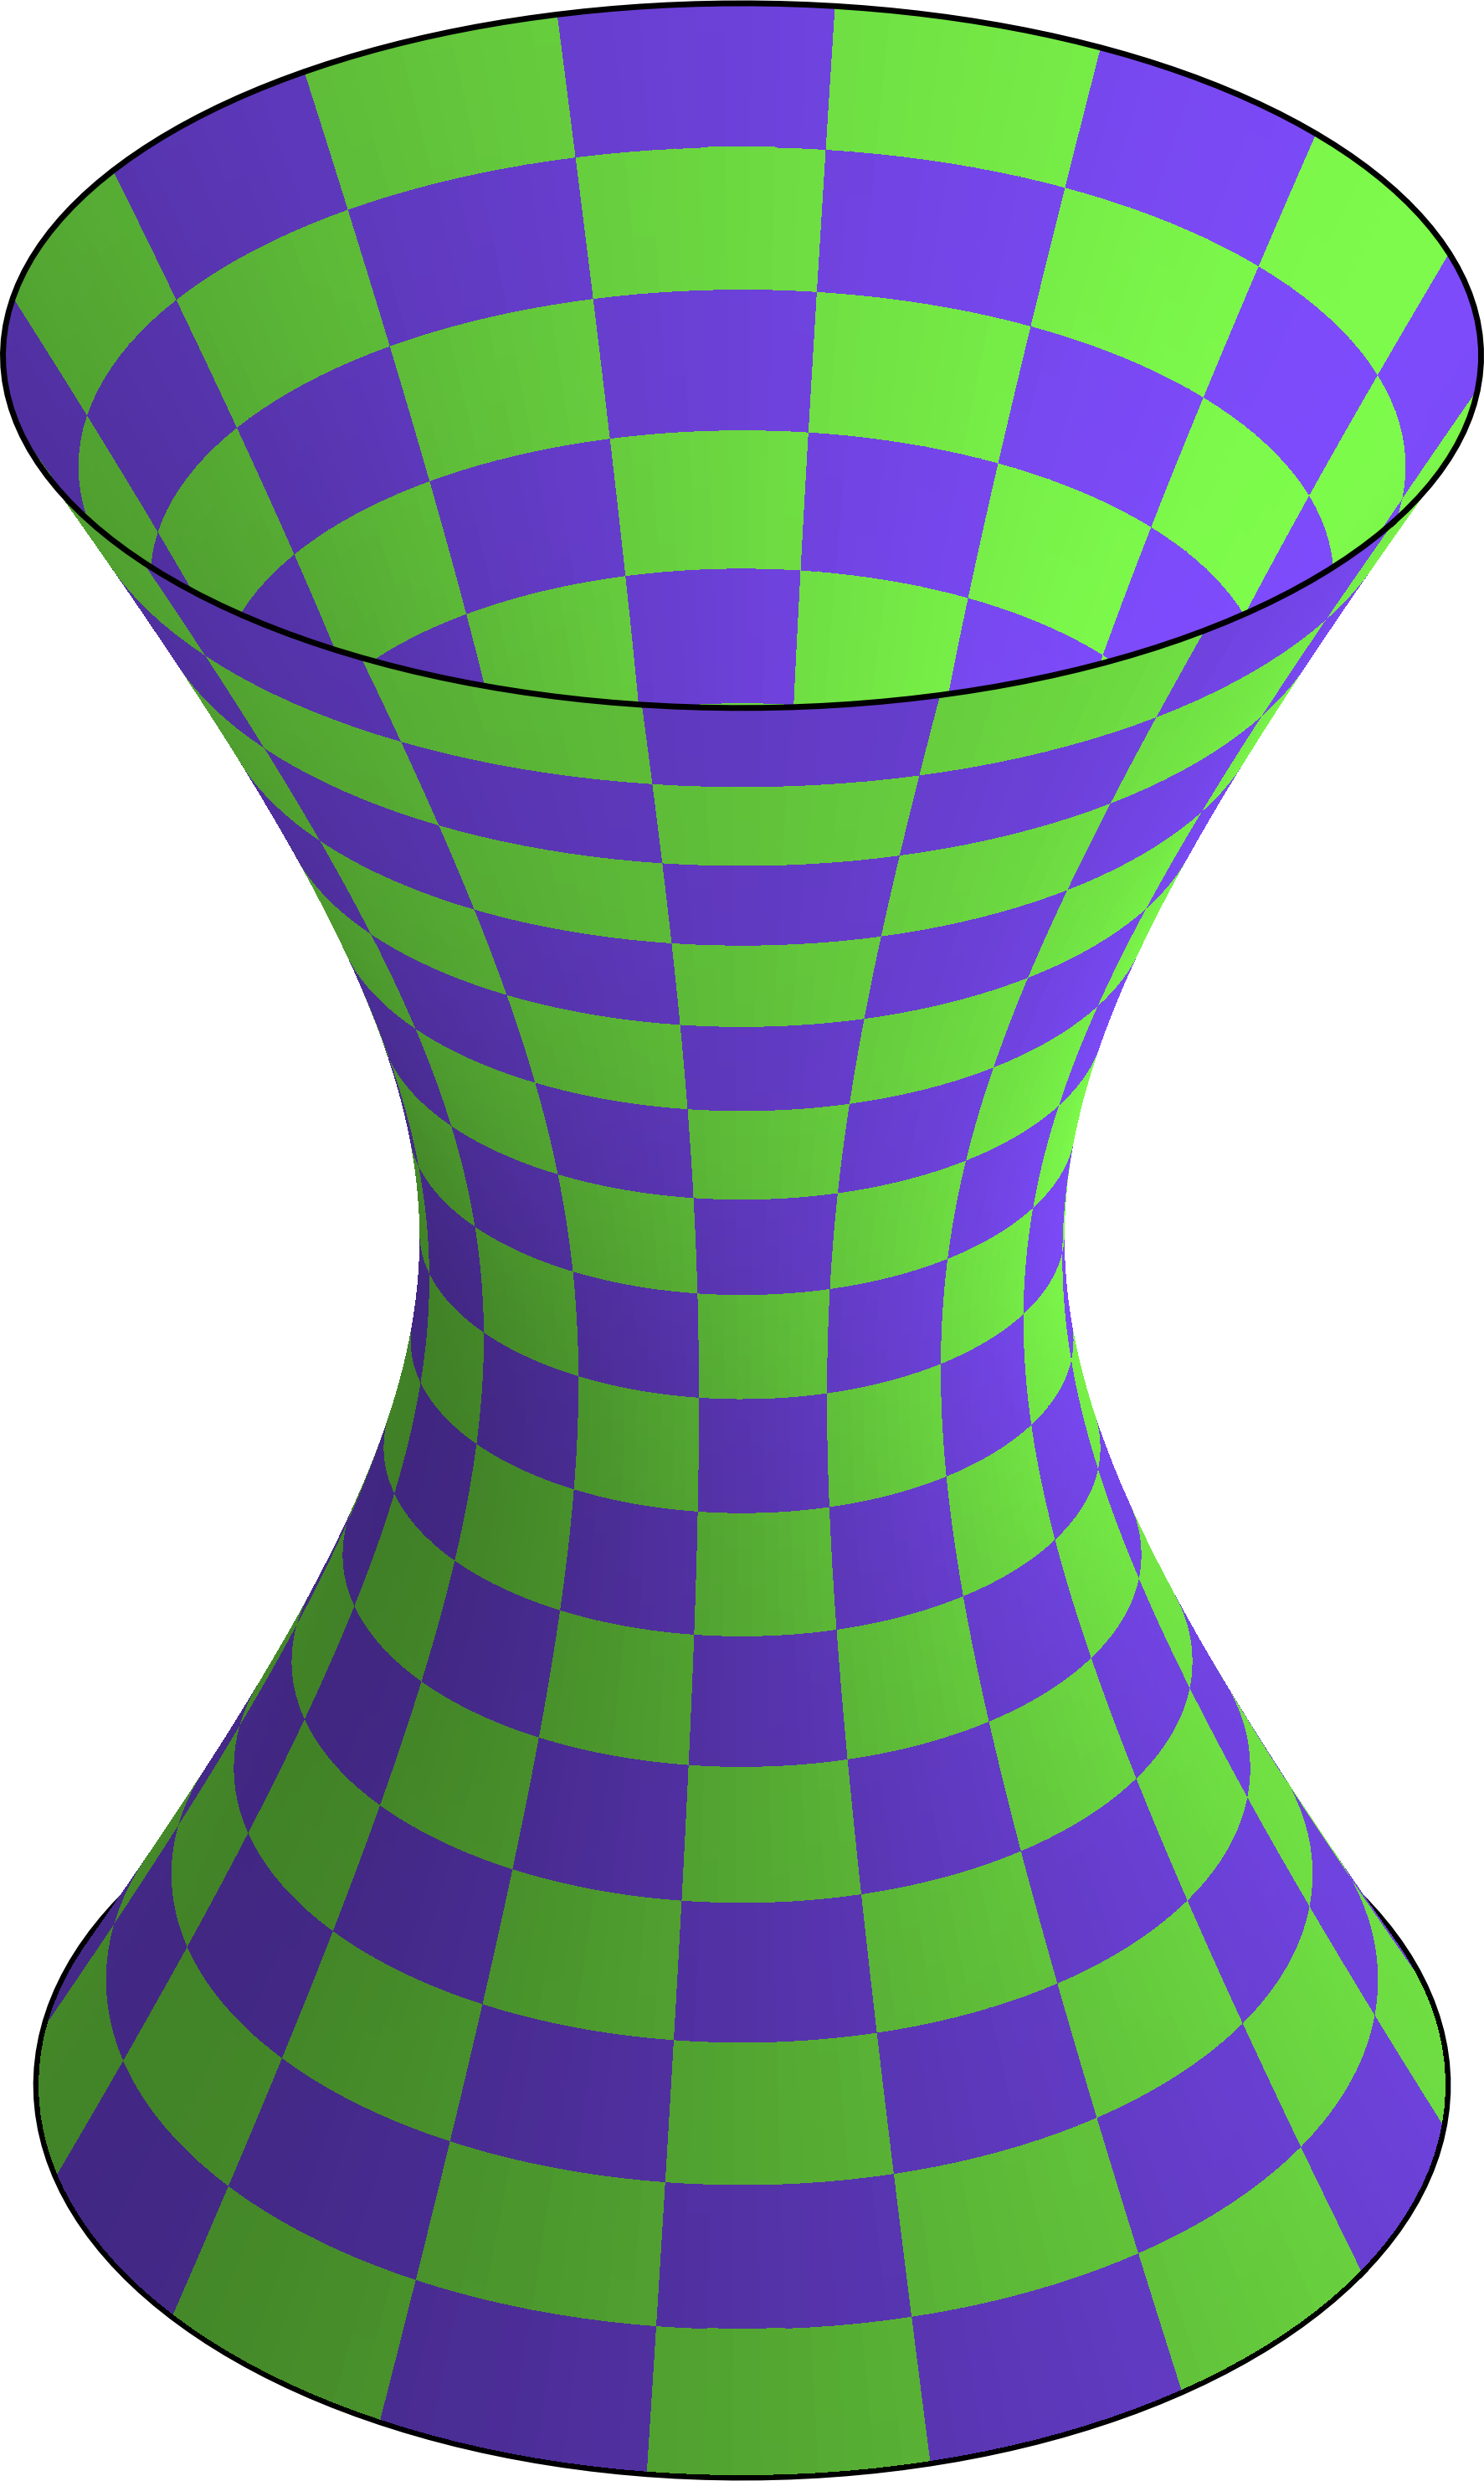
\includegraphics{figs/front}
}
\maketitle

\begin{abstract}
The physics of certain condensed matter systems is not well understood due to strong coupling preventing perturbative descriptions and in certain cases also numerical simulations.
The AdS/CFT correspondence might allow a non-perturbative description of these systems in terms of a dual weakly coupled system. In this thesis the AdS/CFT correspondence is used to model a high-$T_c$ superconductor by a gravity theory outside a black hole in AdS space. The frequency dependent conductivity is calculated using this model and a superconducting phase is shown to appear below a critical temperature.
These computations are described in detail in the first part of the thesis. 
In the second part of the thesis, a higher curvature correction is included on the gravity side in the spirit of effective field theory.
The correction is shown to give a Drude peak and its properties are examined.
Another way to introduce a Drude peak is by introducing a periodic lattice \cite{horowitz}, as was recently done by Horowitz et al. Our way of obtaining the Drude peak is computationally much simpler than the periodic lattice and might be a useful effective description.
\end{abstract}

\section*{Acknowledgements}
Thanks Mum.
\tableofcontents
\chapter{Introduction}
The AdS/CFT correspondence was conjectured in 1997 by Juan Maldacena. It relates the physics of a string theory in Anti de Sitter space (AdS) to a conformal field theory (CFT) on the boundary of the AdS space.\\

AdS is the maximally symmetric space of constant negative curvature. AdS spaces have many interesting properties which will not be described here in detail. A visualization of a two-dimensional AdS space can be made by embedding it as a hyperbola in a three-dimensional space-time with two time directions. The inherited metric is then that of two-dimensional AdS-space with one time direction. See figure on the front of this report. The two time directions span the horizontal plane in this figure. This embedding gives a periodic time which is not necessary. AdS space has, as opposed to Minkowski space, a boundary at spatial infinity. This boundary, often called the \emph{conformal boundary}, can be reached by a massless particle in finite time and boundary conditions must be specified here for a field theory in AdS space. The action of the isometry group of AdS space on the conformal boundary is the conformal group, thereof the name.\\

The string theory in the AdS space is gravitational and thus perturbs the AdS space. The correspondence only requires an asymptotically AdS space. The boundary of the AdS space where the CFT lives is a Minkowski space of one spatial dimension lower. This difference in dimension is why this approach is called \emph{holographic}. The AdS isometry group requires conformal symmetry of the boundary theory which thus is a conformal field theory.
A conformal field theory is a quantum field theory with invariance under conformal transformations. The conformal group is the Poincar\'{e} group with dilations and special conformal transformations added. Dilations are scaling transformations. The word \emph{conformal} comes from the angle-preserving property of these transformations.\\

There is no proof of the correspondence but it has been extensively tested. The field theory of the original conjecture \cite{Maldacena:1997re} was a supersymmetric Yang-Mills theory. Extensions of the conjecture have later been made and we will here use a field theory without supersymmetry. That the extended correspondence also holds is motivated in for example \cite{McGreevy:2009xe}.\\

The strength of the duality comes from that the bulk theory is weakly coupled when the boundary theory is strongly coupled and vice versa. This lets us solve otherwise computationally untractable problems on the strongly coupled side by solving them on the weakly coupled side.\\

%\begin{figure}
%\centering
% 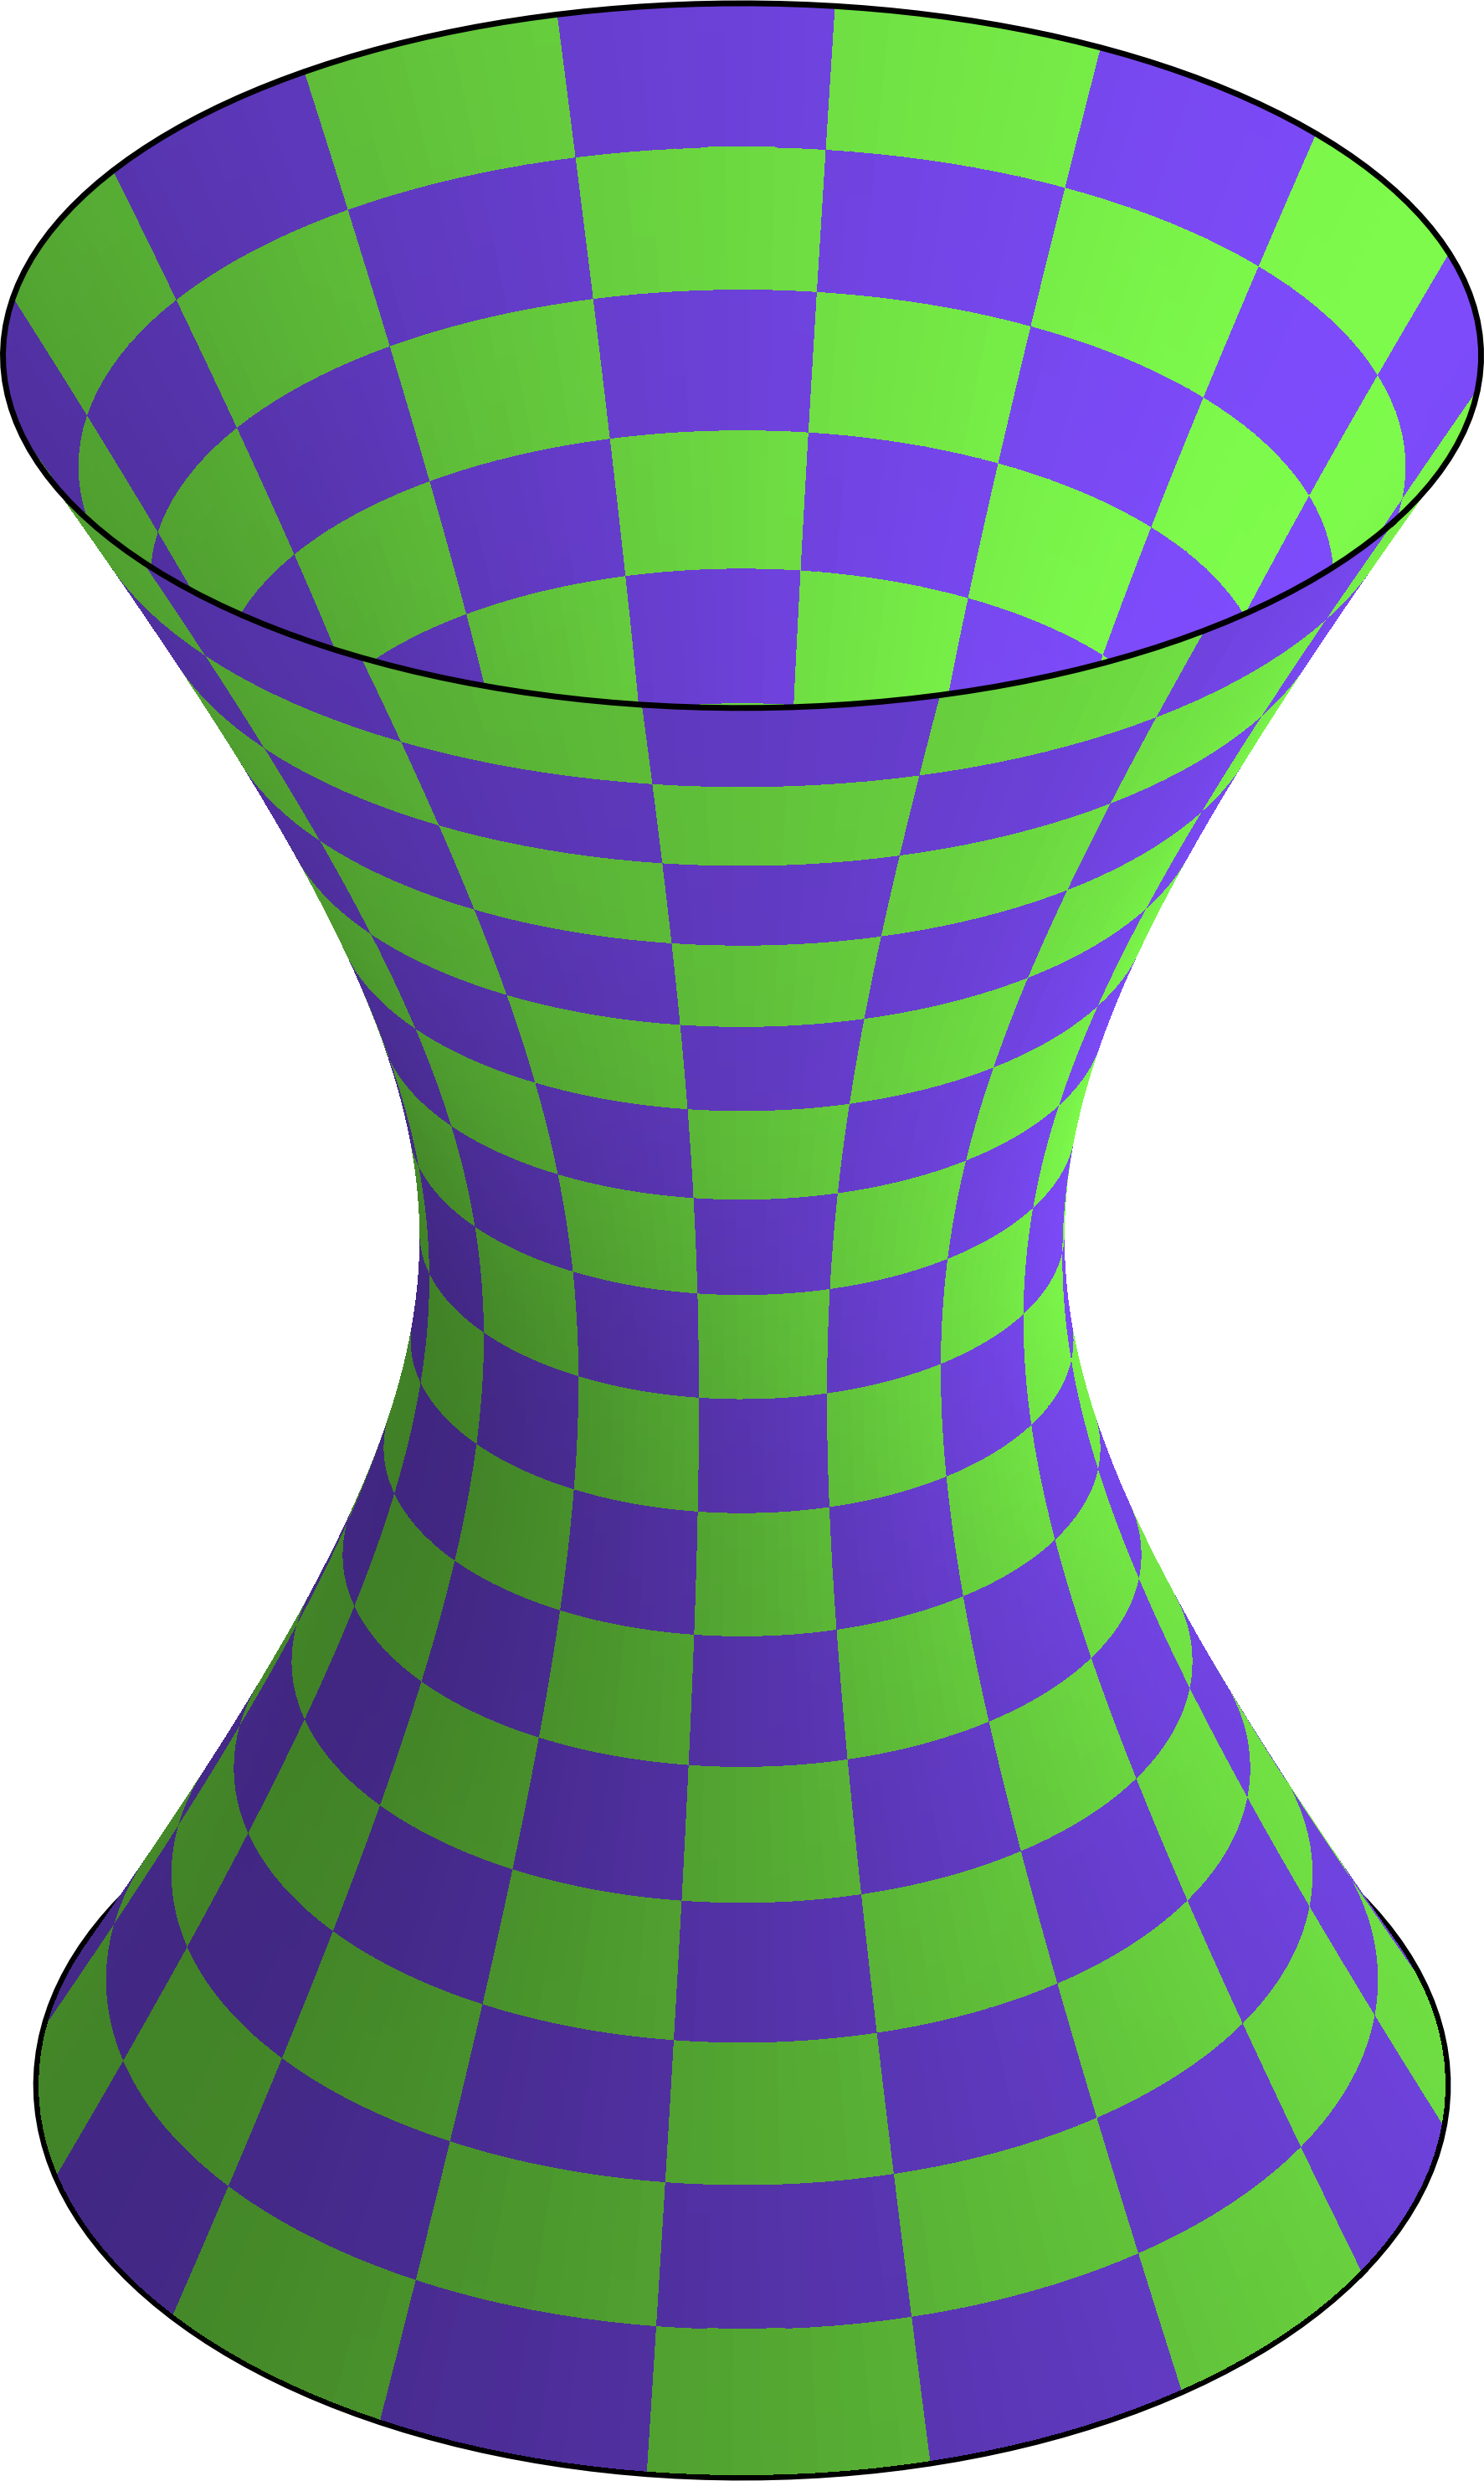
\includegraphics{figs/front}
%\caption{Two-dimensional AdS-space embedded in three-dimensional flat space with two time directions in the %horizontal plane.\label{emb}}
%\end{figure}

\section{The Correspondence\label{correspondence}}
The correspondence can be formulated through
\begin{equation}
 Z_{\mathrm{bulk}}(\delta\psi_{(0)})=\left\langle\exp(\i\int\d^dx\sqrt{g_0}\delta\psi_{(0)}\mathcal{O})\right\rangle_{\mathrm{CFT}}\label{fulCorr}
\end{equation}
 \cite{hartnoll8}. Here $Z_{bulk}(\psi_{(0)})$ is the partition function for the bulk theory with boundary condition\footnote{The boundary condition for the bulk field $\psi$ also includes a power-law scaling towards the boundary, $\psi_{(0)}$ is the factor in front of this scaling. The boundary behaviour of bulk fields will be investigated in Section \ref{s:bb}.} $\psi_{(0)}$ at the conformal boundary.\\

The expectation value on the right-hand side is of a field theory at a temperature given by the Euclidean time periodicity of the path integral for the partition function. The boundary background field $\psi_{(0)}$ is source of the operator $\mathcal{O}$,
\begin{equation}
\mathcal{O}= \frac{\delta S_{\mathrm{CFT}}}{\delta \psi_{(0)}}
\end{equation}
 where $S_{\mathrm{CFT}}$ is the CFT action.\\% The bulk theory contains a field $\psi$ which has a leading boundary behaviour
% \begin{equation}
%  \psi=
% \end{equation}

The bulk theory becomes classical for a boundary gauge theory with a large number of colors, a large $N$. We do not have a large-$N$ theory but a similar effect is expected for certain strongly coupled boundary theories\footnote{The ratio of the AdS-radius $L$ and the gravitational constant $G_N$ act as an effective $N$, $L^{d-1}/G_N=N^2$ \cite{McGreevy:2009xe}. Here $d$ is the dimension of the CFT. This $N$ will be large since we treat the gravity theory in the limit $G_N\rightarrow 0$.} so a classical bulk theory is assummed. See for example \cite{McGreevy:2009xe} for a thorough treatment of when the bulk theory can be considered classical. The partition function is then given in a semi-classical limit by
\begin{equation}
 Z_{\mathrm{bulk}}(\psi_{(0)})=C\exp(\i S_c)\label{semi}
\end{equation}
where $S_c$ is the bulk theory action for the classical periodic path in Euclidean time and $C$ is a constant \cite{hartnoll8}. This path has boundary condition at the conformal boundary described by $\psi_{(0)}$.\\
Expectation values of the CFT operator $\mathcal{O}(x)$ can be calculated by
\begin{equation}
\begin{split}
\frac{\delta S_c(\psi_{(0)})}{\delta\psi_{(0)}(x)}|_{\psi_{(0)}=0}&=
-\i\frac{\delta\log Z_{\mathrm{bulk}}(\psi_{(0)})}{\delta\psi_{(0)}(x)}|_{\psi_{(0)}=0}\\
&=-\i\frac{\delta\log\left\langle\exp(\i\int\d^dx\sqrt{g_{(0)}}\psi_{(0)}\mathcal{O})\right\rangle_{\mathrm{CFT}}}{\delta\psi_{(0)}(x)}|_{\psi_{(0)}=0}\\
&=\frac{\left\langle\mathcal{O}(x)\exp(\i\int\d^dx\sqrt{g_{(0)}}\psi_{(0)}\mathcal{O})\right\rangle_{\mathrm{CFT}}}{\left\langle\exp(\i\int\d^dx\sqrt{g_{(0)}}\psi_{(0)}\mathcal{O})\right\rangle_{\mathrm{CFT}}}|_{\psi_{(0)}=0}\\
&=\langle \mathcal{O}(x) \rangle_{\mathrm{CFT}}
\end{split}
\end{equation}
where the first equality comes from the semi-classical approximation \eqref{semi} and the second equality comes from the correspondence \eqref{fulCorr}. The same correspondence holds for tensor fields with more indices. We have for a vector field $A_a$ that source $J^a$
\begin{equation}
J^a= \frac{\delta S_{\mathrm{CFT}}}{\delta A_{(0)a}}
\end{equation}
the following scheme for extracting a CFT expectation value from the classical bulk
\begin{equation}
\langle J(x)\rangle_{\mathrm{CFT}}=\frac{\delta S_c(\psi_0)}{\delta A_{(0)a}(x)}|_{A_{(0)a}=0}.
\end{equation}\\
The functional derivative needed to calculate these CFT expectation values is the change in total on-shell action when the boundary value of the source field is changed. This can in the case of the operator $\mathcal{O}$ and the source $\psi$ be calculated as follows. All fields of the on-shell bulk theory are in general changed by a change of a boundary value. Denote all the fields in the bulk theory by $\psi_i$. The bulk action $S_c$ is made up of two parts, a bulk Lagrangian density $\L$ and possibly a boundary term with a boundary density $\L_{\mathrm{bdy}}$.
\begin{equation}
 %S_c=\int \d^{d}y\sqrt{g_{(0)}}\L_{\mathrm{bdy}}+\int \d^{d+1}y\sqrt{g}\L
S_c=S_{\mathrm{bdy}}+\int \d^{d+1}y\sqrt{g}\L
\end{equation}
The derivative becomes
\begin{equation}
\begin{split}
\frac{\delta S_c(\psi_{(0)})}{\delta \psi_{(0)}(x)}|_{\psi_{(0)}=0}=&\int \d^{d+1}y\sqrt{g}\left(\frac{\partial\L(y)}{\partial \psi_i(y)}\frac{\partial \psi_i(y)}{\partial \psi_{(0)}(x)}+\frac{\partial\L(y)}{\partial (\nabla_a\psi_i(y))}\frac{\partial (\nabla_a\psi_i(y))}{\partial \psi_{(0)}(x)}\right)\\
&+\frac{\delta S_{\mathrm{bdy}}}{\delta \psi_{(0)}(x)}|_{\psi_{(0)}=0},
%&+\int \d^{d}y\sqrt{g_{(0)}}\left(\frac{\partial\L_{\mathrm{bdy}}(y)}{\partial \psi_i(y)}\frac{\partial \psi_i(y)}{\partial \psi_{(0)}(x)}+\frac{\partial\L_{\mathrm{bdy}}(y)}{\partial (\nabla_a\psi_i(y))}\frac{\partial (\nabla_a\psi_i(y))}{\partial \psi_{(0)}(x)}\right)
\end{split}
\end{equation}
where $i$ goes over all fields and summation is implied. Here the bulk Lagrangian is assumed to only depend on the fields and their first derivatives. Now integrate by parts
\begin{equation}
\begin{split}
\frac{\delta S_c(\psi_{(0)})}{\delta \psi_{(0)}(x)}|_{\psi_{(0)}=0}=&\int \d^{d+1}y\sqrt{g}\left(\frac{\partial\L(y)}{\partial \psi_i(y)}-\nabla_a\frac{\partial\L(y)}{\partial (\nabla_a\psi_i(y))}\right)\frac{\partial \psi_i(y)}{\partial \psi_{(0)}(x)}\\
+&\int_{\partial\mathrm{AdS}} \d^{d}y\sqrt{g_{(0)}}n_a\frac{\partial\L(y)}{\partial (\nabla_a\psi_i(y))}\frac{\partial \psi_i(y)}{\partial \psi_{(0)}(x)}+\frac{\delta S_{\mathrm{bdy}}}{\delta \psi_{(0)}(x)}|_{\psi_{(0)}=0},
\end{split}
\end{equation}
where $n_a$ is an outward normal to the boundary of AdS.
The first integral vanishes since the fields obey the Euler-Lagrange equation. The CFT expectation value can thus be read off from the boundary behaviour of the bulk fields through this relation
\begin{equation}
\begin{split}
\langle\mathcal{O}\rangle_{\mathrm{CFT}}=&\int_{\partial\mathrm{AdS}} \d^{d}y\sqrt{g_{(0)}}n_a\frac{\partial\L(y)}{\partial (\nabla_a\psi_i(y))}\frac{\partial \psi_i(y)}{\partial \psi_{(0)}(x)}+\frac{\delta S_{\mathrm{bdy}}}{\delta \psi_{(0)}(x)}|_{\psi_{(0)}=0}.\label{expFromBdy}
\end{split}
\end{equation}
A CFT expectation value can in this way be obtained from each of the bulk fields once the boundary behaviour of the on-shell bulk fields are known. This also works for tensor fields. This relation will be used in the coming chapters but the boundary behaviour of the bulk fields must first be found.
% The correspondence can be formulated by the GKPW equation \cite{Witten:1998qj}
% \begin{equation}
%  Z_{\text{CFT}}(h)=Z_{\text{strings}}(h)
% \label{GKPW}
% \end{equation}
% where $Z_{\text{CFT}}(h)$ is the partition function of the boundary theory and $Z_{\text{strings}}(h)$ is the partition function of the bulk string-theory. The exact relation between the Lagrangians of the theories is unknown. That the conformal structure fo the two theories are the same 
% 
% Fields in the boundary theory correspond to fields in the bulk theory of same spin.\\
% The boundary theory being scale invariant has different scalings for different operators. Consider an operator $\mathcal{O}$. Scaling the boundary ...TODO
% %but the boundary values of fields in the bulk theory correspond to fields in the CFT.
% TODO
% Lorentz invariance, relativity, causality, locality?


% 
% The boundary values of the bulk fields correspond to fields in the CFT. Expectation values of observables in the CFT can be calculated using a generating functional $Z[J]$. This is a partition function for a system with a perturbed Lagrangian $\L_J(x)=\L(x)+J(x)\mathcal{O}(x)$. Here $\mathcal{O}(x)$ is a local operator on the fields. The generating functional can be regarded an expectation value of a system with the original Lagrangian $\L$.
% \begin{equation}
% \begin{split}
%  Z[J]&=\int_0^{-\i\beta} \mathcal{D}[\psi(t)]\e^{\i \int (\L(\psi(x))+J(x)\mathcal{O}(\psi(x))})\\
% &=Z[0]\int_0^{-\i\beta} \mathcal{D}[\psi(t)]\frac{\e^{\i\int \L(\psi(x))}}{Z[0]}\e^{\i\int J(x)\mathcal{O}(\psi(x))}\\
% &=Z[0]\langle\e^{\i\int J(x)\mathcal{O}(\psi(x))}\rangle
% \end{split}
% \end{equation}
% Taking a functional derivative of this gives:
% \begin{equation}
% \begin{split}
%  \frac{\delta}{\delta J(x)}\log(Z[J])|_{J=0}&=\frac{Z[0]\langle-\i\i \mathcal{O}(\psi(x))\e^{\i\int J(x)\mathcal{O}(\psi(x))}\rangle}{  Z[0]\langle\e^{\i \int J(x)\mathcal{O}(\psi(x))}\rangle }\big |_{J=0}\\
% &= \langle \mathcal{O}(\psi(x))\rangle\label{expectation}
% \end{split}
% \end{equation}
% The partition functions of the bulk and boundary theories are the same even for a perturbed Lagrangian. Both Lagrangians are then perturbed. Expectation values of operators of the boundary theory can thus be calculated using the partition function for the bulk theory. %It is though not trivial to figure out what fields in the bulk theory corresponds to what operators in the boundary theory. 
% %The next chapter will show how to solve the bulk theory and obtain CFT observables.
\section{Applications}
The correspondence can be used both ways but we will consider a strongly coupled boundary theory. Conformal field theories are characterised by not having any specific length scale. Physics at critical points often have this property. A critical point can be a thermodynamic phase transition or a quantum phase transition. The characteristic length goes to infinity as the critical point is approached and the length scale disappears. The physics near a critical point can be expected to be similar to the critical system and finding the critical behaviour is then of interest.\\

Examples of strongly coupled systems exhibiting critical behaviour are, quark-gluon plasmas \cite{PhysRevD.73.045013}, high $T_c$ superconductors \cite{hartnoll8}, and possibly graphene \cite{hartnoll8}.\\

We will hereafter focus on high $T_c$ superconductors. These superconductors are in general layered and the electrons effectively moves in two dimensions. There is no accepted theory describing them possibly due to strong coupling making a theoretical understanding hard. The high $T_c$ supercondictors might be in the vicinity of a quantum critical point \cite{dome} and therefore exhibiting scale-invariance motivating the use of a CFT.

\chapter{Application to Two-Dimensional Condensed Matter Systems}
We wish to model a high $T_c$ superconductor. Conventional superconductors are well described by the BCS theory where the electrons, photons and phonons are the degrees of freedom of interest. The importance of the phonon interactions was understood from the isotope effect, the mass of the atoms in the lattice changed the superconductivity behavior. The isotope effect is though much weaker \cite{leggett2006we}, in high temperature superconductors and the phonons are thus not believed to be important for high temperature superconductivity. The important degrees of freedom are the electrons and the photons. The electrons are, just as in BCS theory, expected to form Cooper-pairs, \cite{leggett2006we}. These are pairs of electrons of opposite spin but otherwise in the same state effectively becoming spin 0 particles. Our high temperature superconductor model will thus contain two fields, a spin 1 field $A_a$ for the photons and a spin 0 field $\psi$ for the Cooper-pairs.\\

The superconductor lives in 2+1 dimensional flat space. We will use coordinates $x$, $y$ for the spatial directions and $t$ for time. The extra dimension in the AdS dual will be parametrised by the coordinate $z$. See Appendix \ref{conventions} for details on how indices are labeled and ordered in this report. 
\section{Symmetry Assumptions}
The bulk theory should have the same symmetries as the boundary theory. We therefore impose a U(1) gauge symmetry of the complex $\psi$ field. Lorentz invariance will also be used for both theories even though relativistic phenomena hardly are important for superconductivity.

\section{A Lagrangian}
There are many different ways to construct a bulk Lagrangian for the fields $A_a$ and  $\psi$ and the metric $g_{ab}$. A Lagrangian previously used succesfully to model two-dimensional electron condensates \cite{hartnoll9, horowitz} will initially be used here.
\begin{eqnarray}
 \mathcal{L}=&\frac{1}{2\kappa}\left(R-2\Lambda\right)-\frac{1}{4}F_{ab}F^{ab}-m^2|\psi|^2-|D_a\psi|^2
\label{L}
\end{eqnarray}
This is obtained using Wilsonian naturalness meaning that the lowest order terms obeying all symmetries are used. A higher order term will be investigated in Chapter \ref{higherOrder}.\\

The action $S$ is calculated from this Lagrangian as
\begin{equation}
 S=\int\d^{d+1} x\sqrt{g}\L+S_\mathrm{boundary}.
\end{equation}
where $g$ is the absolute value of the determinant of the metric tensor, $g=|\det g_{ab}|$. $S_\mathrm{boundary}$ is a boundary term that is needed to cancel divergences when integrating the action towards the boundary. It does not affect the equations of motion but is needed to get normaliseable modes.\\

The first term of the Lagrangian is an Einstein-Hilbert term with a cosmological constant $\Lambda$. A negative cosmological constant gives an asymptotically anti-de-Sitter space as required. $R$ is the Ricci scalar curvature obtained from the metric $g_{ab}$. The constant $\kappa$, proportional to Newton's constant $G_N$, determines the coupling between the metric and the other fields.\\

The second term is an ordinary Maxwell term where the electromagnetic tensor $F_{ab}$ is the exterior derivative of the electromagnetic field tensor, $F_{ab}=\partial_aA_b-\partial_bA_a$.\\

The third and fourth terms are the kinetic and mass terms for the scalar field respectively. $\nabla_a$ is the covariant derivative, see Appendix \ref{conventions}. $D_a$ is the gauge covariant derivative $D_a=\nabla_a-iqA_a$. This minimal gauge coupling makes the Lagrangian invariant under a U(1) gauge transformation
\begin{eqnarray}
 \psi&\rightarrow&\mathrm{e}^{i\theta(x)}\psi\\
 A_a&\rightarrow& A_a+\frac{1}{q}\nabla_a\theta(x)\label{Agauge}.
\end{eqnarray}
%This Lagrangian also possesses conformal invariance. This means that the Lagrangian is unchanged by the transformation $g_{ab}\rightarrow f(x)g_{ab}$. TODO check.
The Lagrangian is also manifestly Lorentz invariant imposing Lorentz invariance of the boundary theory.

\section{Equations of Motion}
The bulk equations of motion are obtained by varying the bulk Lagrangian with respect to all the fields. This can be done with the Euler-Lagrange equation since the action does not contain any higher derivatives. The Euler-Lagrange equation for a scalar field $\chi$ states that
\begin{equation}
 \nabla_a\left(\frac{\partial\mathcal{L}}{\partial(\nabla_a\chi)}\right)-\frac{\partial\mathcal{L}}{\partial\chi}=0.
\end{equation}
First vary $\psi$. This gives
\begin{equation}
\begin{split}
\left(m^2-\nabla^2+q^2A^2+\i q(\nabla_aA^a)\right)\psi&=0.
\end{split}
\end{equation}
Varying $A_a$ gives these equations of motion
\begin{equation}
 -\nabla_aF^{ab}+2q^2|\psi|^2A^b+iq\left(\overline{\psi}\nabla^b\psi-\psi\nabla^b\overline{\psi}\right)=0.
\end{equation}
A real $\psi$ simplifies calculations and that can be obtained since the gauge invariance lets us relate any configuration to a real one through a gauge transformation. The Lorentz gauge,
\begin{equation}
 \nabla_aA^a=0\label{lorentz},
\end{equation}
removes the last term in the parenthesis of the equation of motion for $\psi$. The equation of motion for $\psi$ does not mix the real and imaginary parts after this choice and $\psi$ can be taken to be real since a global shift of phase does not affect $A_a$, see \eqref{Agauge}. The gauge is still not completely fixed, a gauge transformation $\theta(x)$ such that $\nabla_a\nabla^a\theta(x)=0$ can still be done without violating the gauge condition, \eqref{lorentz}. The equations of motion are
\begin{equation}
\begin{split}
\left(m^2-\nabla^2+q^2A^2\right)\psi&=0\\
-\nabla_aF^{ab}+2q^2\psi^2A^b&=0.
\end{split}\label{eqm}
\end{equation}
after choosing the Lorentz gauge and a real $\psi$.
\section{Parameters}
There are multiple free parameters in the bulk Lagrangian. These must be investigated to find values that give us the boundary theory we are interested in. The Lagrangian contains the parameters $\kappa$, $\Lambda$, $m^2$, $q$. Some of these parameters might be redundant since we can make different symmetry transformations of fields and coordinates. The physics of the bulk are treated in the classical limit and the Lagrangian can thus be changed as long as the equations of motion for $\psi$ and $A_a$ are left unchanged.
\subsection{$\kappa$\label{s:kappa}}
The Einstein-Hilbert term of the Lagrangian makes the theory gravitational. $\kappa$ is proportional to Newton's gravitational constant. A small $\kappa$ gives the probe limit where the metric equations of motion can be solved independently of the other fields. This can be understood by varying the Lagrangian with respect to the metric; the Einstein-Hilbert part gives a term inversely proportional to $\kappa$ and the rest of the Lagrangian gives the stress-energy tensor independent of $\kappa$.\\

This greatly simplifies calculations and will therefore be used throughout this work. It is though not guaranteed that the interesting boundary theories are dual to bulk theories in the probe limit. Earlier studies have though found that interesting boundary systems can be obtained by treating a bulk in the probe limit. A superconducting condensate developes for low temperatures in the work by S. Hartnoll, C. Herzog and G. Horowitz \cite{hartnoll9} where the bulk is treated in the probe limit. $\kappa\rightarrow0$ is a fixed-point of the theory so the physics is independent of the exact value of $\kappa$ as long as we are in the probe limit.
\subsection{$\Lambda$}
Scale-invariance of the system lets us choose an arbitrary $\Lambda$. Two systems with different $\Lambda$ can be shown to be equal by a rescaling. $\Lambda$ sets a length scale $L$
\begin{equation}
L=\sqrt{-\frac{3}{\Lambda}}
\end{equation}
to which other parameters, e.g $m^2$, can be related. Scale-invariance can thus not be used to choose those parameters freely. The factor 3 is used so that, as we will later see, $L$ becomes the AdS radius.\\

$\Lambda$ will be set to a convenient number in numerical calculations but kept in calculations for clarity.
\subsection{$q$}
$q$ sets the strength of the gauge coupling and is thus the charge of the scalar field. Considering $\tilde{\psi}=q\psi$ and $\tilde{A}_a=qA_a$ as the fields gives a Lagrangian of the same form but divided by $q^2$ except for the term originally containing $q^2$ which is divided by $q^4$. Multiplying the Lagrangian by a constant doesn't affect the equations of motion so the system can be solved for any value of $q$. Other solutions can then be obtained by rescaling the fields.\\
\subsection{$m^2$}
$m$ is the mass of the scalar field in the bulk. What values of $m$ that are suitable will be investigated later when solving the equations of motion in the bulk.



% \section{Partition Function}
% The partition function is a concept from statistical physics. It is for a quantum-mechanical system defined as
% \begin{equation}
%  Z(\beta)=\mathrm{tr}(\e^{-\beta\hat{H}})
% \end{equation}
% where $\hat{H}$ is the time-independent Hamiltonian and $\beta=(k_BT)^{-1}$ where $k_B$ is Boltzmann's constant and $T$ is the temperature. Hereafter we let $k_B=1$ meaning that we measure temperature in units of what energy it corresponds to. The partition function is similar to the trace of the time-evolution operator $\hat{U}(t_2,t_1)$ evolving a state from time $t_1$ to $t_2$
% \begin{equation}
%  \mathrm{tr}(\hat{U}(t_2,t_1))=\mathrm{tr}(\e^{-\i\frac{(t_2-t_1)\hat{H}}{\hbar}})=f(t_2-t_1).
% \end{equation}
% We will hereafter let $\hbar=1$ by measuring energy in units of inverse time. The partition function can be obtained as the analytical extension of $f$,
% \begin{equation}
%  Z(\beta)=f(-\i\beta).
% \end{equation}
% The trace of the time evolution operator can be calculated as an integral over configuration space which in our case will be field configurations $\Psi$,
% \begin{equation}
%  f(t)=\int \mathcal{D}[\Psi] \bracket{\Psi}{\hat{U}(t,0)}{\Psi}.
% \end{equation}
% The time-evolution operator matrix elements can be calculated using Feynman's path integrals \cite{feynman1965quantum},
% \begin{equation}
%  \bracket{\Psi_2}{\hat{U}(t,0)}{\Psi_1}=\int_{\Psi_1}^{\Psi_2} \mathcal{D}[\Psi(t)]\e^{\i S[\Psi(t)]}
% \end{equation}
% where $S[\Psi(t)]$ is the action of the path $\Psi(t)$ through field configurations. Combining these results tells us that the trace $f(t)$ can be calculated as a periodic time path integral with period $t$
% \begin{equation}
%  f(t)=\int_0^t \mathcal{D}[\Psi(t)]\e^{\i S[\Psi(t)]}.
% \end{equation}
% This means that $Z(\beta)$ can be obtained by calculating a path integral where the time is imaginary and periodic. The action must be analytically extended to imaginary time $\tau=\i t$. 
% %\begin{equation}
% % S[\Psi(\tau)]=\int_0^\beta\d \tau\int\d x\sqrt{g} \L(\Psi(\tau),\Psi^\prime(\tau),...)
% %\end{equation}
% The metric of the CFT is the metric induced from the bulk theory. The boundary is time-like and the time periodicity of the two theories are thus the same. This means that they are at the same temperatures. The path integral can for a classical theory be calculated using the saddle point approximation. The partition function is then
% \begin{equation}
%  Z(\beta)=f(-\i\beta)\stackrel{\mathrm{classical}}{=} \e^{ \i S_c}\label{classical}
% \end{equation}
% where $S_c$ is the on-shell action for a periodic path with period $-\i\beta$. For a solution stationary in time the action is $S_c=-\i\beta L_c$ where $L_c$ is the imaginary time saddle-point Lagrangian. The classical partition function then becomes
% \begin{equation}
%  Z(\beta)= \e^{\beta L_c}\label{classical2}
% \end{equation}

\chapter{Solution of the Classical Bulk Theory}
We wish to compute expectation values of the CFT. This will be done through the correspondence using relation \eqref{expFromBdy}. The bulk theory equations of motion must then be solved so that the boundary behaviour of the fields can be obtained.
%The bulk theory was assumed to be classical in Section \ref{correspondence} so the system is solved by finding the equations of motion for the fields and solving them. This lets ut calculate the partition function and use it to find CFT expectation values through \ref{expectation}.
\section{Definitions}
The Lagrangian describes a general system so there are many solutions to the equations of motion. We wish to investigate two properties of a superconductor, the development of a condensate at low temperatures and the conductivity at different frequencies. We are interested in a superconductor subject to spatially uniform conditions, the applied electric field is uniform and the chemical potential is uniform. The atomic lattice and its imperfections are thus not accounted for but interesting superconductivity behaviour has been obtained anyway \cite{hartnoll9}. It is thus enough to look at a system with translational symmetry in the $x$ and $y$ directions. A rotationally invariant superconductor will further be studied. The system is subject to conditions constant in time, e.g.~no time-dependent chemical potential. This lets us assume time-independence while solving the non-linear field equations.\\

The conductivity is the linear electrical current response to an applied transverse electrical field. We can apply this in the $x$ direction due to the rotational symmetry. We let the applied field have a harmonic time dependence $\exp(\i t \omega)$ so we can get the response function in the frequency domain. The linear response is sought so the applied field should be infinitesimal. The applied field breaks the rotational and time symmetries but since it is infinitesimal and we are not interested in the effect is has on the other fields it can be neglected while calculating them. The applied field is later added with the other fields as a background solution.\\
The electrical field in the $x$-direction is $E_x=F_{xt}=\nabla_xA^t-\nabla_tA^x$. Translational symmetry gives $E_x=\nabla_tA^x$.

These limitations lets us do the following definitions
\begin{equation}
 \begin{split}
  \d s^2&=g_{tt}(z)\d t^2+g_{zz}(z)\d z^2+g_{xx}(z)(\d x^2+\d y^2)  \\
  \psi&=\psi(z)\\
  A_a&=(\At(z), A_z(z), A_x(z)\exp(\i t \omega), 0)
 \end{split}\label{defs}
\end{equation}
where $\At(z)$ is infinitesimal.
The gauge condition requires
\begin{equation}
 \nabla_aA^a=\partial_aA^a+\Gamma^a_{\ ba}A^b=0
\end{equation}
this gives a homogeneous first-order linear ordinary differential equation for $A_z(z)$ since the contracted Christoffel symbol only has a $z$ component. The remaining gauge symmetry lets us add a function to $A_z$ and can be used to set $A_z(z)=0$ for a $z$. The above differential equation then requires $A_z(z)$ to be identically 0 for all $z$. We will hereafter work with $A_z(z)=0$.\\

The explicit $z$ and $t$-dependence of these functions will hereafter be ommited. 
\section{Metric\label{s:metric}}
The path integral for the bulk partition function is approximated in a semi-classical approximation where we need the saddle-point of the action. We first wish to find the \emph{metric} saddle-point of the periodic imaginary time path integral. The bulk equation of motion for the metric $g_{ab}$ is the Einstein equation with a cosmological constant
\begin{equation}
R_{ab}-\frac{1}{2}g_{ab}R+g_{ab}\lambda=\kappa T_{ab}\label{einstein}
\end{equation}
where $R_{ab}$ is the Ricci curvature tensor and $T_{ab}$ is the stress-energy tensor. We assumed the probe limit in Section \ref{s:kappa} and therefore neglect the right hand side of this equation. We want a translationally invariant solution in the $t$, $x$, and $y$ directions that is asymptotically AdS. The solution is known to be a black hole \cite{McGreevy:2009xe}, the Schwarzschild metric in AdS space. The metric has the following form in a particular choice of coordinates where the radial coordinate $z$ is 0 at the boundary and $z_h$ at the horizon
\begin{equation}
 g_{ab}\d x^a\d x^b=\frac{L^2}{z^2}\left(\frac{\d z^2}{f(z)}-f(z)\d t^2+\d x^2+\d y^2\right).\label{metric}
\end{equation}
Here $f(z)=1-z^3z_h^{-3}$. $f(z)$ approaches 1 at the boundary and the space is asymptotically AdS. There is a horizon at $z=z_h$ where $f(z_h)=0$. The space behind the horizon can not affect the physics of the boundary and can thus be neglected in our calculations. This solution is periodic in imaginary time. Consider the near-horizon metric where
\begin{equation}
  f(z)=f(z_h)-(z_h-z)f'(z_h)+\mathcal{O}((z_h-z)^2)\approx 3(1-zz_h^{-1})
\end{equation}
Do the change of variables $\rho^2=\frac{4L^2}{3}(1-zz_h^{-1})$. This gives $f(z)\approx \rho^2\frac{9}{4L^2}$ and $\rho^2\d \rho^2=\d z^2 z_h^{-2}\frac{4L^4}{9}$. The near-horizon metric is then
\begin{equation}
\begin{split}
 g_{ab}\d x^a\d x^b&=\frac{L^2}{z_h^2}\left(\frac{\rho^2\d \rho^2  }{z_h^{-2}\frac{4L^4}{9}\rho^2\frac{9}{4L^2}}-\rho^2\frac{9}{4L^2}\d t^2+\d x^2+\d y^2\right)\\
&= \d \rho^2 -\rho^2\frac{9}{4z_h^2}\d t^2+\frac{L^2}{z_h^2}\left(\d x^2+\d y^2\right).
\end{split}
\end{equation}
Now extend this to imaginary time $\tau=\i t$
\begin{equation}
\begin{split}
 g_{ab}\d x^a\d x^b
&= \d \rho^2 +\rho^2\left(\frac{3}{2z_h}\d \tau\right)^2+\frac{L^2}{z_h^2}\left(\d x^2+\d y^2\right).
\end{split}
\end{equation}
The near horizon metric is then that of a Euclidean plane in polar coordinates. There is thus a deficit angle unless $\frac{3}{2z_h}\tau$ has a periodicity of $2\pi$. The imaginary time has periodicity $\beta$ so we thus have
\begin{equation}
 \frac{3}{2z_h}=\frac{2\pi}{\beta}
\end{equation}
This gives the relationship between $z_h$ and the temperature
\begin{equation}
 T=\frac{3}{4\pi  z_h}\label{T}.
\end{equation}
This expression for the temperature agrees with the Beckenstein-Hawking temperature of a black hole.\\

The backreaction $\delta g_{ab}$ from the non-zero fields will be of order $\kappa T_{ab}$ according to \eqref{einstein}. The Einstein equation is obtained by varying the Lagrangian with respect to $g_{ab}$ so $\delta S\propto\kappa^{-1}\delta g_{ab}^2$ for the solution. We thus have that $\delta S\propto\kappa T_{ab}^2$ and the backreaction can safely be neglected also when calculating the action from different field configurations.\\

This background metric can now be used instead of solving the equations of motion for the metric together with the fields. The gravitational part of the Lagrangian must be kept when calculating the value of the total action which is dominated by the gravitational part.
% The Ricci scalar of the solution metric is
% \begin{equation}
%  R=-\frac{d(d+1)}{L^2}=2\Lambda\frac{d+1}{d-1}
% \end{equation}
% where the boundary dimension $d$ has been kept for clarity. The action can be calculated using this. A Gibbons-Hawking-York boundary term is needed in addition to the Einstein-Hilbert term \cite{PhysRevD.15.2752}, \cite{PhysRevLett.28.1082} since we have a boundary with Dirichlet boundary conditions. The boundary term is
% \begin{equation}
%  S_{\mathrm{grav}}=\frac{1}{2\kappa}\int \d^{d+1}x\sqrt{-g}\left(R-2\Lambda\right)-\frac{1}{\kappa}\int \d^dx\sqrt{\gamma}\left(-\gamma^{ab}\nabla_an_b+\frac{d-1}{L}\right)
% \end{equation}
% where $n_a$ is a normal vector at the boundary. 
%  Consider the space $(z,t,\mathbf{x})\in[\epsilon,z_h]\times V$ corresponding to a $d$-volume of the boundary theory $V$. The action boundary density is then
% \begin{equation}
% \begin{split}
%  \frac{S_{\mathrm{grav}}}{V}&=\frac{\Lambda}{\kappa}\left(\frac{d+1}{d-1}-1\right)\int_\epsilon^{z_h}\d z\sqrt{-g}+
% \frac{1}{\kappa}\sqrt{\gamma}\left(-\gamma^{ab}\partial_a\d z_b+\frac{d-1}{L}\right)\\
% &=\frac{\Lambda}{\kappa}\frac{2}{d-1}\int_\epsilon^{z_h}\d z\left(\frac{L}{z}\right)^{d+1}+
% \frac{1}{\kappa}\left(\frac{\epsilon}{L}\right)^{-d}\frac{d-1}{L}\\
% &=\frac{L\Lambda}{\kappa}\frac{2}{d(d-1)}\left(\left(\frac{\epsilon}{L}\right)^{-d}-\left(\frac{z}{L}\right)^{-d}\right)\\
% &=-\frac{1}{L\kappa}\left(\left(\frac{\epsilon}{L}\right)^{-d}-\left(\frac{z_h}{L}\right)^{-d}\right)
% \end{split}
% \end{equation}
% The total action density is obtained as $\epsilon\rightarrow0$.

The horizon $z_h$ and the curvature length $L$ set length scales in the metric. Length units in the numerical solution can be chosen such that $z_h=1$. This means that we for different temperatures have different units since $z_h$ is related to the temperature. We will have to convert between these units when comparing results from different temperatures.\\

%This $T$ in units of energy is also in units of inverse length since we chose the energy unit to the inverse time it 
\section{Field Equations of Motion}
The equations of motion for $\psi(z)$, $\At(z)$ and $A_x(z)$ can now be obtained. Inserting \eqref{defs} into the equations of motion \eqref{eqm} and using the metric \eqref{metric} gives
\begin{empheq}[left=\empheqlbrace]{align}
 &\Big(q^2z^2\phi^2-L^2m^2f+zf(zf^\prime-2f)\partial_z+z^2f^2\partial_z\partial_z\Big)\psi=0\label{eqm1}\\
 &\Big(-2q^2\psi^2L^2+z^2f\partial_z\partial_z\Big)\phi=0\\
 &\Big(-2q^2\psi^2L^2f+z^2\omega^2+z^2ff^\prime\partial_z+z^2f^2\partial_z\partial_z\Big)A_x=0\label{eqm3}
\end{empheq}
The formulas in Appendix \ref{CAS} have here been used.
\subsection{Field behaviour at Conformal Boundary\label{s:bb}}
A Frobenious expansion \cite{teschl2012ordinary} of these equations can be done at the boundary, $z=0$. The leading behaviour of the functions is
\begin{empheq}[left=\empheqlbrace]{align}
 &\psi=\psi_{(0)}\left(\frac{z}{z_h}\right)^{\Delta_\psi}\\
 &\phi=\phi_{(0)}\left(\frac{z}{z_h}\right)^{\Delta_\phi}\\
 &A_x=A_{x(0)}\left(\frac{z}{z_h}\right)^{\Delta_{A_x}}
\end{empheq}
where $\Delta_\psi$, $\Delta_\phi$ and $\Delta_{A_x}$ are constants that are to be determined. This is a slight assumption since not all functions have this type of leading behaviour.
 Entering this in the equations of motion yields
 \begin{empheq}[left=\empheqlbrace]{align}
  &q^2z^2\phi_{(0)}^2s^{2\Delta_\phi}-L^2m^2f+f(zf^\prime-2f)\Delta_\psi+f^2\Delta_\psi(\Delta_\psi-1) =0\label{ind1}\\
  &-2q^2\psi_{(0)}^2s^{2\Delta_\psi}L^2+f\Delta_\phi(\Delta_\phi-1)=0\label{ind2}\\
  &-2q^2\psi_{(0)}^2s^{2\Delta_\psi}L^2f+z^2\omega^2+zff^\prime\Delta_{A_x}+f^2\Delta_{A_x}(\Delta_{A_x}-1)=0.
 \end{empheq}
where $s=zz_h^{-1}$. This immidiately gives $\Delta_\psi\geq0$ and $1+\Delta_\phi\geq0$ since the first terms otherwise diverges at the horizon where the other terms are finite. First consider the case of the strict inequalities. The leading order behaviour is then
 \begin{empheq}[left=\empheqlbrace]{align}
  &-L^2m^2-2\Delta_\psi+\Delta_\psi(\Delta_\psi-1) =0\\
  &\Delta_\phi(\Delta_\phi-1)=0\\
  &\Delta_{A_x}(\Delta_{A_x}-1)=0.
 \end{empheq}
with solutions
 \begin{empheq}[left=\empheqlbrace]{align}
  &\Delta_\psi =\frac{3}{2}\pm\sqrt{\frac{9}{4}+L^2m^2}\label{indicialSo1}\\
  &\Delta_\phi=0,1\\
  &\Delta_{A_x}=0,1\label{indicialSol3}.
 \end{empheq}
Now assume $\Delta_\psi=0$. \eqref{ind2} gives
\begin{equation}
 -2q^2\psi_{(0)}^2L^2+\Delta_\phi(\Delta_\phi-1)=0
\end{equation}
while \eqref{ind1} gives $\Delta_\phi=-1$. We then have
 \begin{empheq}[left=\empheqlbrace]{align}
  &q^2\phi_{(0)}^2z_h^{2} =L^2m^2\label{spurious1}\\
  &q^2\psi_{(0)}^2L^2=1\\
  &\Delta_{A_x}(\Delta_{A_x}-1)=2.
 \end{empheq}
with solutions $\Delta_{A_x}=-1,2$.
First assuming $\Delta_\phi=-1$ yields the same result. There are though no solutions to \eqref{spurious1} for the negative $m^2$ we later will consider and infinities are encountered when calculating the action for these solutions so they will not be considered.
All useful solutions are thus given by equation \ref{indicialSo1} to \ref{indicialSol3}.
\subsection{Field behaviour at Horizon\label{s:hb}}
The same kind of expansion can be made at the horizon but there are some simplifying conditions. The time component of the metric vanishes at the horizon, $f(z_h)=0$. This means that $A_t(z_h)$ must be zero because a finite $A_t(z_h)$ would give a finite Wilson loop around the periodic imaginary time circle whose length in time is 0. A Wilson loop is contrary to $A_t$ a physical quantity ($A_t$ is gauge-dependent). This gives a singular gauge connection which is unphysical \cite{hartnoll8}. We thus have $\At(z_h)=0$. Expand the fields as 
\begin{empheq}[left=\empheqlbrace]{align}
 &\psi=\psi_{(h)}s^{\Delta^{(h)}_\psi}\\
 &\phi=\phi_{(h)}s^{\Delta^{(h)}_\phi}\\
 &A_x=A_{x(h)}s^{\Delta^{(h)}_{A_x}}
\end{empheq}
where $s$ now is $(1-z/z_h)$ and $\Delta^{(h)}_\phi>0$. The notation $\Delta^{(h)}$ is used to signify that these exponents describe the \emph{horizon} behaviour, $\Delta$ was earlier used for the conformal boundary behaviour. The function $f$ can be expanded as $f=3s-3s^2+s^3$.
% \begin{empheq}[left=\empheqlbrace]{align}
%  &q^2z^2\phi_{(1)}^2s^{2\Delta^{(h)}_\phi}-L^2m^2f-zf(zf^\prime-2f)s^{-1}\Delta^{(h)}_\psi+z^2f^2s^{-2}\Delta^{(h)}_\psi(\Delta^{(h)}_\psi-1)=0\\
%  &-2q^2\psi_{(1)}^2s^{2\Delta^{(h)}_\psi}L^2+z^2fs^{-2}\Delta^{(h)}_\phi(\Delta^{(h)}_\phi-1)=0\\
%  &-2q^2\psi_{(1)}^2s^{2\Delta^{(h)}_\psi}L^2f+z^2\omega^2-z^2ff^\prime s^{-1}\Delta^{(h)}_{A_x}+z^2f^2s^{-2}\Delta^{(h)}_{A_x}(\Delta^{(h)}_{A_x}-1)=0
% \end{empheq}
Insert these leading terms in the equations of motion. We get
\begin{empheq}[left=\empheqlbrace]{align}
 &q^2z^2\phi_{(h)}^2s^{2\Delta^{(h)}_\phi}+9z_h^2\Delta^{(h)}_\psi+z_h^2 9\Delta^{(h)}_\psi(\Delta^{(h)}_\psi-1)=0\\
 &-2q^2\psi_{(h)}^2s^{2\Delta^{(h)}_\psi}L^2+z_h^2 3s^{-1}\Delta^{(h)}_\phi(\Delta^{(h)}_\phi-1)=0\\
 &-6q^2\psi_{(h)}^2s^{2\Delta^{(h)}_\psi+1}L^2+z_h^2\omega^2+ 9\Delta^{(h)}_{A_x}+9\Delta^{(h)}_{A_x}(\Delta^{(h)}_{A_x}-1)=0.
\end{empheq}
Solving for the leading terms of these equations gives
% \begin{empheq}[left=\empheqlbrace]{align}
%  &\Delta^{(h)}_\psi=0\\
%  &\Delta^{(h)}_\phi(\Delta^{(h)}_\phi-1)=0\\
%  &\omega^2+  9\Delta^{(h)}_{A_x}^2=0.
% \end{empheq}
% This has solutions
\begin{empheq}[left=\empheqlbrace]{align}
 &\Delta^{(h)}_\psi=0\\
 &\Delta^{(h)}_\phi=1\\
 &\Delta^{(h)}_{A_x}=\pm\frac{\i\omega z_h}{3}\label{inout}.
\end{empheq}
The two possible $\Delta^{(h)}_{A_x}$ represent solutions going into or coming out of the horizon. Close to the horizon is $A_x(z,t)$ given by
\begin{equation}
 A_x(z,t)=s^{\pm\frac{\i\omega z_h}{3}}\exp(\i\omega t)=\exp\big(\i\omega(t\pm\frac{z_h\log s}{3})\big).
\end{equation}
The phase is constant for $s=\exp(\mp3t/z_h)$ so the plus sign in \eqref{inout} gives the ingoing solution.

\subsection{Boundary Conditions}
The equations of motion, \eqref{eqm1} to \eqref{eqm3}, can be integrated numerically. Just one leading horizon behaviour is allowed for $\psi$ and $\At$ so only two horizon conditions are needed for them, $\psi(z_h)$ and $\At'(z_h)$. The derivative $\psi'(z_h)$ needed for starting a numerical integration from the horizon can be obtained directly from the equations of motion as $z\rightarrow0$
\begin{equation}
 \psi'(z_h)=-\frac{L^2m^2}{3z_h}.
\end{equation}
A two parameter family of solutions to the equations of motion can then be obtained for $\psi$ and $\At$. These solutions give the boundary values of the fields which describe the background fields of the field theory. The two horizon parameters must be choosen to obtain the desired background fields.\\

The field theory operator $\mathcal{O}$ corresponding to the background field $\psi$ is expected to \emph{spontaneously} attain a non-zero expectation value breaking the U(1) symmetry. We therefore require the source $\psi_{(0)}=0$.\\

The time component of the electromagnetic potential $A_a$ corresponds to the electrical potential in the Lorentz gauge. The electrical potential gives the energy per charge needed to add a charge to the system and the chemical potential for the electrons $\mu$ can thus be expressed as $\mu=q\phi_{(0)}$.\\

Just one of the two horizon behaviours of the Maxwell perturbation $A_x$ is wanted. We want a casual response from the perturbation of the background field. This corresponds to the solution going \emph{into} the horizon as time passes \cite{hartnoll8}. We thus choose the ingoing horizon behaviour. The equation for $A_x$ is linear and we are only interested in the linear response at the conformal boudary so the horizon amplitude of the ingoing solution can be choosen arbitrarily.\\

The horizon parameters $\psi(z_h)$ and $\At'(z_h)$ can now be varied to find solutions to the two boundary conditions $\psi_{(0)}=0$ and $\mu=q\phi_{(0)}$. See Appendix \ref{a:num} for a description of the numerical integration. The Maxwell perturbation can afterwards be integrated from the horizon to the boundary for a range of values of $\omega$.\\

There is a trivial analytical solution of the equations of motion with the above boundary conditions.
\begin{equation}
\begin{split}
 &\psi(z)=0\\
 &\phi(z)=\mu(1-z/z_h)\\
 &A_x(z)=
\left[
\exp\left( - \sqrt{3}\tan^{-1} \frac{z_h+2z}{z_h\sqrt{3}} \right)
\frac{z_h-z}{\sqrt{z^2+zz_h+z_h^2}}
\right]^{\frac{\i\omega z_h}{3} }   \label{trivial}
\end{split}
\end{equation}
The field $\psi$ is here identically zero and there is no spontanous symmetry breaking. This solution thus corresponds to the physics above the critical temperature, $T_c$, of the superconductor. We will now make a choice of $m$ to be able to investigate solutions with $\psi\neq0$
\subsection{Choice of scalar mass $m$}
The mass squared of a scalar field in flat space must be non-negative for stability. This is though not the case in a space with negative curvature. The Breitenlohner-Freedman bound (BF) is a lower bound on $m^2$ of a massive scalar field in AdS space with metric given by \eqref{metric}. It requires
\begin{equation}
 L^2m^2\geq-\frac{d^2}{4}\label{BF}
\end{equation}
for stability\cite{Kleban:2004bv}. The scalar field $\psi$ should obey this bound far away from the black-hole for normaliseable modes. We would though like a spontanous symmetry breaking of $\psi$ near the black hole\footnote{The physics close to the black hole in the bulk corresponds to low energy physics of the boundary theory, see e.g.~\cite{McGreevy:2009xe}.} corresponding to the electron condensate \cite{Gubser:2008px}. This can happen because the coupling of $\psi$ to $A_a$ gives $\psi$ an effective mass that might break the BF bound near the black hole. \\The effective mass is given by:
\begin{equation}
 m_{\mathrm{eff}}^2=m^2+A_aA^a
%=m^2+g^{tt}\At^2
=m^2-\frac{z^2}{L^2(1-z^dz_h^{-d})}\At^2
\label{meff}
\end{equation}
This can for large enough values of $\At$ break the BF-bound, see Fig. \ref{BF}.
\begin{figure}
\centering
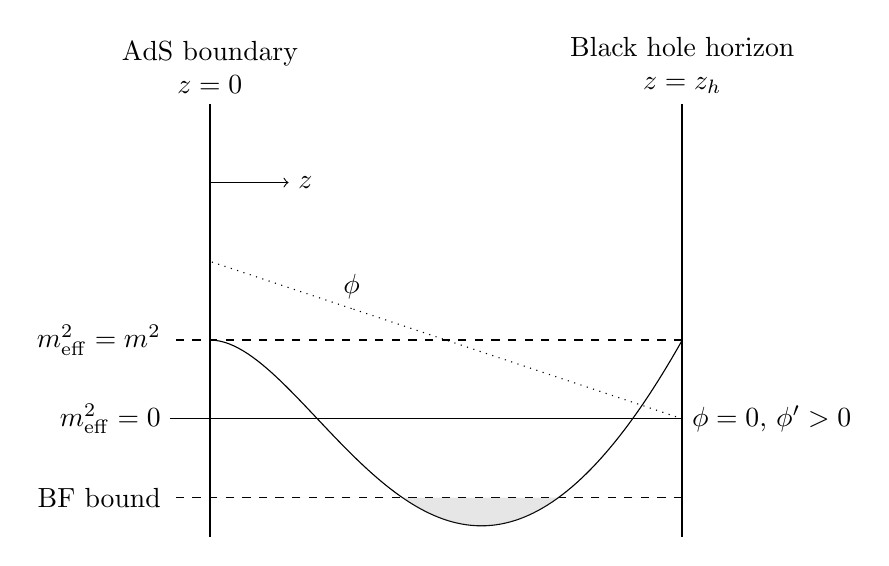
\begin{tikzpicture}
    \draw[->] (0,3) -- (1,3) node[right] {$z$};
    \draw[-,thick] (0,-1.5) -- (0,4) node[above,align=center] {AdS boundary\\$z=0$};
    \draw[-,thick] (6,-1.5) -- (6,4) node[above,align=center] {Black hole horizon\\$z=z_h$};
    \draw[-] (6,0) -- (-0.5,0) node[left] {$m_{\mathrm{eff}}^2=0$};
    \draw[-] (6,1) -- (-0.5,1)[dashed] node[left] {$m_{\mathrm{eff}}^2=m^2$};
    \draw[-] (6,-1) -- (-0.5,-1)[dashed] node[left] {BF bound};
    \draw[dotted] plot[domain=1:0.3,samples=50] (\x*6,{2*(1-\x)})node[above] {$\phi$};
    \draw[dotted] plot[domain=0.3:0,samples=50] (\x*6,{2*(1-\x)});
    \draw[-] (6,0) node[right] {$\phi=0$, $\phi^\prime>0$};
    \draw[solid] plot[domain=0:1,samples=100] (\x*6,{1-2*\x*\x/(1-\x*\x*\x)*4*(1-\x)*4*(1-\x)});
    \draw [fill=gray,fill opacity=0.2,draw=none] plot[domain=0:1,samples=100] (\x*6,{-1}) -- plot[domain=0:1,samples=100] (\x*6,{min(1-2*\x*\x/(1-\x*\x*\x)*4*(1-\x)*4*(1-\x),-1)});
\end{tikzpicture}
\caption{Schematic plot of how the the effective mass breaks the BF bound outside the horizon. A value of $\At$ has been assumed.\label{BF}}
\end{figure}
Consider the trivial, uncondensed, solution \eqref{trivial}. When does this give an effective mass breaking the BF-bound and possibly enabling an additional condensed solution? The location of the effective mass minimum, $z_0$, can be found by differentiating \eqref{meff} by $z$ and using \eqref{trivial},
\begin{equation}
\frac{z_0}{z_h}=\frac{1}{3} \left(\sqrt[3]{37+9 \sqrt{17}}-\frac{2}{\sqrt[3]{37+9 \sqrt{17}}}-2\right).
\end{equation}
The effective mass breaks the BF-bound at $z_0$ when
\begin{equation}
 \frac{\mu}{T}>
\frac{2\pi }{\sqrt{3}} \sqrt{\frac{4 L^2 m^2+9}{8-\sqrt[3]{142-34
   \sqrt{17}}-\sqrt[3]{142+34 \sqrt{17}}}}
\end{equation}
where \eqref{T} has been used. We will, following \cite{hartnoll8, horowitz}, choose $m^2L^2=-2$. This does not break the BF bound but it is relatively close. It gives integer scalings for the scalar field at the conformal boundary which is convenient.%Write about near horizon AdS geometry instead and ...?
\section{Expectation Values of Field Theory Operators}
Expectation values of field theory operators can now be calculated using these solutions and \eqref{expFromBdy}. Not just the leading behaviour of the fields is needed to calculate the expectation values but also the first subleading behaviour. Therefore we expand the fields as
\begin{empheq}[left=\empheqlbrace]{align}
 &\psi=\psi_{(0)}\frac{z}{L}+\psi_{(1)}\left(\frac{z}{L}\right)^{2}\\
 &\phi=\phi_{(0)}+\phi_{(1)}\frac{z}{L}\\
 &A_x=A_{x(0)}+A_{x(1)}\frac{z}{L}
\end{empheq}
and obtain $\psi_{(i)}$, $\phi_{(i)}$ and $A_{x(i)}$ from the numerical solution.
For this the boundary terms to the action are required. The boundary term needed for the scalar field is calculated in Appendix \ref{a:bound}.
\begin{equation}
\begin{split}
 S_{\mathrm{bdy}}&=-\int_{z=\epsilon}\d^dxL^{-1}\psi^2\sqrt{g_{(0)}}
\end{split}
\end{equation}
Now insert this in relation \eqref{expFromBdy}
\begin{equation}
\begin{split}
\langle\mathcal{O}\rangle_{\mathrm{CFT}}=&\int_{\partial\mathrm{AdS}} \d^{d}y\sqrt{g_{(0)}}
\left(
n_a\frac{\partial\L(y)}{\partial (\nabla_a\psi(y))}
-2L^{-1}\psi
\right)\frac{\delta \psi(y)}{\delta \psi_{(0)}(x)}=\\
&=
\frac{L^3}{z^3}\left(
\frac{z}{L}2\nabla_z\psi(y)
-2L^{-1}\psi
\right)  \frac{z}{L}\\
&=
\frac{L^2}{z^2}
\left(
\frac{z}{L}2(\psi_{(0)}\frac{1}{L}+\psi_{(1)}\frac{2z}{L^{2}})
-2L^{-1}(\psi_{(0)}\frac{z}{L}+\psi_{(1)}\left(\frac{z}{L}\right)^{2})
\right)  \\
&=
\frac{2\psi_{(1)}}{L}
\end{split}
\end{equation}
This simple relation thus gives us the expectation value of the scalar operator. A similar derivation can be made for the other fields. A general expression is shown in \cite{hartnoll8}, equation 91\footnote{The difference of a factor 2 is due to their kinetic term having a factor $1/2$ we do not.}. We have for the current $J^a$ sourced by the background field $A_a$
\begin{equation}
 \langle J^a\rangle_{\mathrm{CFT}}=A_{a(1)}
\end{equation}
The current gives us the charge density $\rho=-\At_{(1)}$ and the transverse current $J_x=A_{x(1)}$. The minus sign is a convention to get a positive charge density.\\

We are now in a position to numerically solve the bulk theory and obtain these expectation values. We do this by sweeping over different horizon values of $\psi$ and for each value find all solutions to the boundary condition $\psi_{(0)}=0$. This yields many different solutions $\rho/T$ at the boundary. Scale invariance lets us interpret this as systems of constant $\rho$ but at different temperatures $T$. We then get a variation in the chemical potential $\mu$, see Figure \ref{f:mu}. The chemical potential of the trivial solution there shown is calculated through
\begin{equation}
 \rho=\mu/z_h.
\end{equation}
Alternatively one can let $\mu$ be constant while varying the temperature and get a variation in $\rho$. Figure \ref{f:O} shows the expectation value of $\mathcal{O}$ at different temperatures. The solid line at the bottom is the trivial solution $\psi=0$. The temperature $T_c$ is defined as the temperature where the first non-trivial solution is obtained. Multiple solutions are obtained as the temperature is lowered. The different solutions correspond to different phases of the system and which one is physical can be found by finding which has the lowest free energy.

\fig{O_constRho_a2_0.0.pdf}{Expectation value of CFT operator $\mathcal{O}$ at different $T$ and constant $\mu$. The multiple curves correspond to multiple solutions at the same temperature. The dashed lines have negative expectation values of $\mathcal{O}$. Further solutions (here ommited) are obtained for lower temperature following the trend shown here.\label{f:O}}

\fig{mu_constRho_a2_0.0.pdf}{
Chemical potential needed for constant $\rho$ at different $T$. The multiple curves correspond to multiple solutions at the same temperature. The dashed lines have negative expectation values of $\mathcal{O}$. Further solutions (here ommited) are obtained for lower temperature following the trend shown here.\label{f:mu}
}

\section{Free Energy}
The free energy, $A=-T\log{Z}$, is the same for the bulk and the boundary theory since their partition functions are the same. This can be calculated in the classical limit in the bulk.
\begin{equation}
 A=-T\log{Z}\stackrel{\mathrm{classical}}{=}-\i T S_c
\end{equation}
Here $S_c$ is the classical periodic time action. The classical field solutions only depend on the $z$ coordinate and are thus proportional to $V=-\i\beta V_2$ where $V_2$ is the area considered in coordinates $x_1$, $x_2$. This gives the free energy per surface area
\begin{equation}
 \frac{A}{V_2}=-\int_0^{z_h}\d z \sqrt{-g}\L+V^{-1}S_{\mathrm{bdy}}
\end{equation}
%Consider the case where $m^2=-2$. Then $\Delta_0=1$ and the boundary term is given by \eqref{Sbdy}.\\
% \subsection{Gravitational Free Energy and Entropy}
% The action is dominated by the gravitational part since we are in the probe limit. 
% The expression for the temperature \eqref{T} can be used to calculate the free energy from the action at finite temperature
% \begin{equation}
% \begin{split}
%  \frac{A_\mathrm{grav}}{V_2}&=-T\frac{-1}{\kappa}\sqrt{\frac{-2\Lambda}{6}}\left(\frac{3}{4\pi TL}\right)^{-3}\\
% &=\frac{(4\pi)^3T^3L^{2}}{3^{3}\kappa}
% \end{split}
% \end{equation}
% \\
% The entropy $H$ can now be calculated from the free energy
% \begin{equation}
%  H=-\frac{\partial A}{\partial T}=-\frac{(4\pi)^dT^{d-1}L^{d-1}}{d^{d-1}\kappa}.
% \end{equation}
\subsection{Free Energy of Scalar and Electromagnetic Fields}
Only the free energy difference of the different solutions shown in Figure \ref{f:O} is needed. We therefore calculate the free energy contribution from the scalar and electromagnetic fields and neglect the contribution from the Einstein-Hilbert term of the action. We do not need to account for the contribution from any back-reaction on the metric following our argument in Section \ref{s:metric}. First consider the trivial solution \eqref{trivial}.
\begin{equation}
\begin{split}
 \frac{A}{V_\mathrm{2}}=&-\int_0^{z_h}\d z \sqrt{-g}\L+V_\mathrm{2}^{-1}S_{\mathrm{bdy}}\\
=&\int_0^{z_h}\d z \left(\frac{z}{L}\right)^{-4}\frac{1}{4}F_{ab}F^{ab}\\
=&\int_0^{z_h}\d z \left(\frac{z}{L}\right)^{-4}\frac{1}{2}F_{zt}^2g^{zz}g^{tt}\\
=&-\int_0^{z_h}\d z \frac{\mu^2}{2z_h^2}\\
=&-z_h^{-1}\frac{\mu^2}{2}\\
=&-\left(\frac{4\pi T}{3}\right)\frac{\mu^2}{2}
\end{split}
\end{equation}
The free energy for the numerical solutions has been calculated and the result together with this analytical result is shown in Figure \ref{f:A}. It can there be seen that the trivial solution is the physical solution for temperatures above $T_c$ and that the solution appearing at the temperature $T_c$ is the physical solution for all lower temperatures. We will hereafter only work with these two solutions.

\fig{A}{The free energy for the different solutions are shown here for constant $\rho$ and varying $T$. The trivial solution is shown as the thick solid line. The other curves correspond to numerical solutions. The lowest one corresponds to the solution appearing at $T=T_c$ and the other roots follow in order.\label{f:A}}

\section{Electrical Conductivity}
The conductivity of a superconductor can easily be measured experimentally for a wide range of frequencies and it is therefore an interesting property to calculate from our model of a superconductor. The agreement in different frequency ranges tells us about similarities and differences between our model and the experimental superconductors.\\
\subsection{Definition of Electrical Conductivity and its Properties}
We define conductivity $\sigma$ as the linear response function for the current density $J_x$ with the applied electrical field $E_x$ as source
\begin{equation}
 \sigma(\omega)=\frac{J_x(\omega)}{E_x(\omega)}\label{sigma}.
\end{equation}
Here the direction $x$ has been chosen for concreteness but since we consider two-dimensional systems with rotational symmetry we need only consider one direction. These functions of $\omega$ are the Fourier transforms of the time-dependent quantities. The current in the time domain can be obtained from the conductivity and the applied field through a inverse Fourier transform
\begin{equation}
 J_x(t)=\int_{-\infty}^\infty E_x(t-\tau)\sigma(\tau)\d \tau.
\end{equation}
Causality implies that $\sigma(\tau)=0$ for $\tau<0$ since the current would otherwise depend on future values of the electrical field. The conductivity can using this be written
\begin{equation}
 \sigma(\omega)=\int_0^\infty\sigma(\tau)\exp(\i\tau\omega)\d\tau
\end{equation}
and thus has an analytical extension to the upper half of the complex plane. Both the current, $J_x(t)$, and applied field, $E_x(t)$, are real quantities which makes $\sigma(\tau)$ also real and thus $\re(\sigma(w))$ an even function and $\im(\sigma(\omega))$ odd. These properties of $\sigma(\omega)$ give the Kramers–Kronig relations
\begin{equation}
\begin{split}
 \re(\sigma(\omega))&=\frac{2}{\pi}\int_0^\infty\frac{\omega^\prime\im(\sigma(\omega^\prime))}{\omega^{\prime 2}-\omega^2}\\
\im(\sigma(\omega))&=-\frac{2}{\pi}\int_0^\infty\frac{\omega\re(\sigma(\omega^\prime))}{\omega^{\prime 2}-\omega^2}\label{kk}
\end{split}
\end{equation}
These relations state that the real part of the conductivity uniquely determines the imaginary part and vice versa.
\subsection{Calculating the Holographic Conductivity}
We want to apply a homogeneous but time-varying electrical field on the superconductor and measure the induced current. The two-dimensional superconductor is rotationally symmetric so we can apply the field in any direction. We choose
\begin{equation}
 E_x=E_0\exp(-\i\omega t).
\end{equation}
The response function can be obtained by using this time-dependence. This electrical field corresponds to the electromagnetic potential
\begin{equation}
 A=(A_z,\At,A_x,A_y)
\end{equation}


Applying an electric field in 
The obtained conductivity for temperatures above the $T_c$ is $\sigma(\omega)=1$. This agrees with TODO. The conductivity changes when the condensate forms. An energy gap $\Delta$ forms and the conductivity for $\omega<\Delta$ goes to 0 as the temperature is lowered. The superconductivity is not immidiately evident from the obtained conductivity curves. There is a delta-function at $\omega=0$ since translational invariance of the boundary theory has been assumed.
\fig{cond_Ts}{Real and imaginary part of the conductivity for different temperatures. Higher temperatures above $T_c$ give the same conductivity as for the $T=T_c$ case. \label{cond_Ts}}
TODO, add DC temperature dependence? energy gap size?
\subsection{Comparison with Experimental Results}
TODO. graphene?
\section{Consistency Check using a Conductivity Sum Rule}
The Kramers-Kroning relations and the decoupeling of the electrons from the system at high frequencies can be used to prove a sum rule for the conductivity \cite{PhysRev.109.1398}. The rule states
\begin{equation}
 \int_0^\infty\re(\sigma(\omega))\d\omega=C
\end{equation}
where $C$ is a constant depending on what system we are considering 
\fig{sum_rule_a20}{Integral}


\chapter{Extended Lagrangian\label{higherOrder}}
Many assumptions have been made in the previous study. The most simple Lagrangian \eqref{L} has been used and translational symmetry has been assumed. This has given us a boundary theory with a scalar field that condeses below a critical temperature as expected for a superconductor. The conductivity shows both similarities and differences with that of high-$T_c$ superconductors. A $\delta$-function developes at $\omega=0$ for $T<T_c$ giving infinite DC conductivity. An evident difference is the lack of a so-called Drude peak at low frequencies. A Drude peak is an increase in conductivity for low frequencies in metals that can be well modeled by the Drude model of conductivity\cite{drude}, thereof the name. The Drude model agrees with experiments on cuprates above $T_c$\cite{drudeFit}.

\section{Drude Model}
The Drude model is obtained by treating the charge carriers classically. They are expected to obey the differential equation
\begin{equation}
 \frac{\d v}{\d t}=\frac{q}{m}E-\frac{1}{\tau}v
\end{equation}
Solving this for harmonic $E=E_0\exp(-\i\omega t)$ gives 
\begin{equation}
 v=\frac{\tau qE_0}{m(1-\i\omega\tau)}\exp(-\i\omega t).
\end{equation}
This gives the conductivity
\begin{equation}
 \sigma(\omega)=\frac{J(\omega)}{E(\omega)}=\frac{v(\omega)q\rho}{E(\omega)}=\frac{\tau\rho q^2}{m(1-\i\omega\tau)}=\frac{\sigma_0}{1-\i\tau\omega}.
\end{equation}
where $\rho$ is the density of charge carriers of charge $q$.
\section{Higher Order Maxwell Term}
Different generalizations of the standard Lagrangian $L$ have been studied, TODO cite. Tobias Wenger studied three different extensions propose by Sachdev, TODO cite. An increase in conductivity for low frequencies similar to a Drude peak, courtesy of Hugo Strand, was observed for one of the extensions. This will here be studied in more detail.\\
The extended Lagrangian has a higher order Maxwell term and another parameter $\alpha_2$ with dimension TODO.
\begin{eqnarray}
 \mathcal{L}=&\frac{1}{2\kappa}\left(R-2\Lambda\right)-\frac{1}{4}F_{ab}F^{ab}-m^2\psi\overline{\psi}-D_a\psi\overline{D^a\psi}
+\alpha_2F^a_bF^b_cF^c_dF^d_a\label{L2}
\end{eqnarray}
The equations of motion now become TODO.\\
TODO: Boundary, Horizon behaviour.\\

This higher order term introduces a perturbation in the low frequency conductivity above the critical point. The perturbation is very close to what is expected from the Drude model of electrical conductivity. 
This agrees very well with what is obtained for low frequencies above the critical point, especially for high values of TODO. See Fig. \ref{drude}.




\fig{drude_T_1Tc_a2_1}{Conductivity for $\alpha_2=1$ and $T=T_c$. The Drude parameters have been obtained from the lowest frequency data-point. \label{drude}}

The low frequency limit of the conductivity $\sigma_0$ seems to depend linearly on $\alpha_2$ for values of $\alpha_2$ larger than TODO. See Fig \ref{drudeVar2Tc}. The proportionality constant depends on the temperature, see Fig \ref{drudeVarMTc}, and seems to closely follow a power-law, see Fig \ref{drudeTdep_1e4}. $\sigma_0$ thus seems to closely follow
\begin{equation}
 \sigma_0=C\alpha_2\left(\frac{T}{T_c}\right)^{-4/3}
\end{equation}
for values of $\alpha_2>>TODO$.


\section{Asymptotic Behavior for $\alpha_2>>T_c^?$,TODO}
\fig{drudeVar2Tc}{Drude parameters as functions of $\alpha_2$ at $T=2T_c$.\label{drudeVar2Tc}}

\fig{drudeVarMTc}{$\omega\rightarrow0$ limit of the conductivity as a function of $\alpha_2$ for different temperatures.\label{drudeVarMTc}}

\fig{drudeTdep_1e4}{$\sigma_0/\alpha_2$ as a function of temperature for large $\alpha_2$.\label{drudeTdep_1e4}}
\section{Consistency Check using a Conductivity Sum Rule}
A test of the numerics was again performed by verifying the TODO...
\fig{sum_rule_a20}{Integral, TODO plot new}

\section{Disussion}
The peak in the Drude model is due to imperfections in the lattice
\subsection{Comparison with Results using a Periodic Lattice}
TODO
\chapter{Summary}
TODO
\section{Outlook}
TODO
\begin{appendices}
\chapter{Conventions in this Report\label{conventions}}
The AdS space will be refered to as the bulk and the boundary conformal field theory will be referred to as the boundary theory or the superconductor or just CFT. We use $z$ for the ``radial'' coordinate in AdS space, it is 0 at the conformal boundary and $z_h$ at the horizon. This is the same coordinate as the one called $r$ in \cite{hartnoll8}, there with horizon at $r=r_+$.\\
Vector quantities not involving time components will in the boundary theory be written with boldface, $\mathbf{E}, \mathbf{J}$.\\
Tensor indices in the $d+1$-dimensional bulk theory will be TODO latin letters, $a,b,c,...8$. Tensor indices in the $d$-dimensional boundary theory will be TODO greek letters, $\mu,\nu,...$. Tensors written in component form will have it's components ordered as $\mu=t,x,y$ on the boundary and $a=z,t,x,y$ in the bulk.
The metric sign convention for positive space-like distances will be chosen.\\
The action is calculated from the Lagrangian as
\begin{equation}
 S=\int\d^{d+1} x\sqrt{g}\L+S_\mathrm{boundary}.
\end{equation}
This is independent of coordinates but makes us use covariant derivatives for finding the equations of motion. The square root could instead be absorbed in the Lagrangian and the space time be considered flat. This has been done in computer-aided calculations of the equations of motion.
\chapter{Dimensions}
What dimension different variables have can be a bit confusing. Here is a table to clear things up
\begin{equation}
 \begin{split}
[z]&=[L]\\
[m^2]&=[L^{-2}]\\
[q]&=[L^{0}]\\
[\omega]&=[L^{-1}]\\
[\mathcal{L}]&=[L^{-4}]\\
[S]&=[L^0]\\
[T]&=[L^{-1}]\\
[\psi]&=[L^{-1}]\\
[\mathcal{O}]&=[L^{-2}]\\
[A_a]&=[L^{-1}]\\
[F_{ab}]&=[L^{-2}]\\
[J^a]&=[L^{-2}].
 \end{split}
\end{equation}


\chapter{Boundary Term for Scalar Field Action \label{a:bound}}
The bulk Lagrangian considered will contain different fields and depends both on the fields and their first derivatives. Here we will consider a simple Lagrangian with just one scalar field and figure out what boundary term is needed for the Lagrangian.\\

Consider a field $\psi$ with a kinetic term $-(\partial_a\psi)^2$ and a potential term $V(\psi)$. The classical solution is the one that extremises the action. The action integral contains the metric as an integration measure
\begin{equation}
 S=\int\d^{d+1} x\sqrt{|\det g_{ab}|}\L\equiv\int\d^{d+1} x\sqrt{g}\L.
\end{equation}
The Euler-Lagrange equation is obtained by varying the action. The integration measure can then be regarded as part of the Lagrangian or covariant derivatives can be used in the derivation of the Euler-Lagrange equation. The measure becomes when using the metric \eqref{metric} $L^{d+1}z^{-d-1}$. The Euler-Lagrange equation gives
\begin{equation}
\begin{split}
 0=\partial_a\left(\frac{\partial (z^{-d-1}(V(\psi)-(\partial_b\psi)^2)) }{\partial(\partial_a\At)}\right)-\frac{\partial  (z^{-d-1}(V(\psi)-(\partial_b\psi)^2) )}{\partial\At}=\\
 =-\partial_a\left(z^{-d-1}2\partial^a\psi\right)-z^{-d-1}V'(\psi)\\
\end{split}
\end{equation}
We will be interested in boundary systems with translational symmetry so $\psi$ is assumed to be a function of $z$. The equation of motion then becomes
\begin{equation}
\begin{split}
0=-\partial_z\left(z^{-d-1}2g^{zz}\partial_z\psi\right)  -\frac{V'(\psi)}{z^{d+1}}=\\
-\partial_z\left(z^{-d-1}2(z^2L^{-2}f(z))\partial_z\psi\right)  -\frac{V'(\psi)}{z^{d+1}}=\\
-z^{-d-1}2z^2L^{-2}f(z)\psi''-L^{-2}\left((-d+1)z^{-d}2f(z) + z^{-d+1}2f'(z)\right)\psi' -\frac{V'(\psi)}{z^{d+1}}
\end{split}
\end{equation}
This gives a second order differential equation for $\psi(z)$
\begin{equation}
\begin{split}
0=-z^22f(z)\psi''-\left((-d+1)z2f(z) + z^22f'(z)\right)\psi' -L^2V'(\psi)
\end{split}
\end{equation}
Now consider the boundary, $z=0$. Our metric is required to be asymptotically AdS so $f(0)\rightarrow1, zf'(0)\rightarrow0$. $\psi$ can be expanded at the boundary as a Laurent series. Call the lowest exponent in this series $\Delta$. $\psi$ will then behave as $z^\Delta$ near the boundary. This should solve the differential equation in the near boundary limit. Insertion of $z^\Delta$ into the differential equation and taking the limit of small $z$ gives
\begin{equation}
\begin{split}
0&=-z^22\Delta(\Delta-1)z^{\Delta-2}-\left((-d+1)2z + z^22f'(z)\right)\Delta z^{\Delta-1} -L^2V'(z^{\Delta})\\
&=z^{\Delta}\left(-2\Delta(\Delta-1)-2(-d+1)\Delta\right)-L^2V'(z^{\Delta}).
\end{split}
\end{equation}
Now consider a potential for a massive scalar field, $V(\psi)=-m^2\psi^2+\mathcal{O}(\psi^3)$. We then get the following equation for $\Delta$
\begin{equation}
\begin{split}
%0=\Delta(\Delta-1)-(d-1)\Delta-L^2m^2=\\
0=\Delta^2-d\Delta-L^2m^2
\end{split}
\end{equation}
in the limit $z\rightarrow0$. This has solutions
\begin{equation}
\begin{split}
\Delta=\frac{d\pm\sqrt{d^2+4L^2m^2}}{2}.
\end{split}
\end{equation}
$\psi$ thus goes as $z^{\Delta_0}$ where $\Delta_0$ is the smaller solution and $\Delta_1$ the larger. The leading behaviour of $\psi$ near $z=0$ is
\begin{equation}
 \psi=\psi_0\left(\frac{z}{L}\right)^{\Delta_0}+\psi_1\left(\frac{z}{L}\right)^{\Delta_1}
\end{equation}
unless $\Delta_1-\Delta_0>=1$ and further terms from the series corresponding to $\Delta_0$ must be included.\\

What will the contribution to the action from this solution be? Consider the action contribution from the region $z\in[\epsilon,\delta]$ where $\delta$ is small and $\epsilon\rightarrow0$.
\begin{equation}
\begin{split}
 S_{[\epsilon,\delta]}=&\int_{z\in[\epsilon,\delta]}\d^{d+1} x\sqrt{g}\L=\\
=&V\int_\epsilon^\delta\d z \left(\frac{z}{L}\right)^{-d-1}\left(-m^2\psi^2-(\partial_a\psi)^2\right)=\\
=&V\int_\epsilon^\delta\d z \left(\frac{z}{L}\right)^{-d-1}\left(-m^2( \psi_0\left(\frac{z}{L}\right)^{\Delta_0}+\psi_1\left(\frac{z}{L}\right)^{\Delta_1} )^2-(\partial_a(\psi_0\left(\frac{z}{L}\right)^{\Delta_0}+\psi_1\left(\frac{z}{L}\right)^{\Delta_1}))^2\right)=\\
=&V\int_\epsilon^\delta\d z \left(\frac{z}{L}\right)^{-d-1}\Big[-m^2 \left(\psi_0^2\left(\frac{z}{L}\right)^{2\Delta_0}+\psi_1^2\left(\frac{z}{L}\right)^{2\Delta_1}+2\psi_0\psi_1\left(\frac{z}{L}\right)^{\Delta_0+\Delta_1}\right) \\
&-g^{zz}L^{-2}(\Delta_0\psi_0\left(\frac{z}{L}\right)^{\Delta_0-1}+\Delta_1\psi_1\left(\frac{z}{L}\right)^{\Delta_1-1})^2\Big]=\\
=&V\int_\epsilon^\delta\d z\left(\frac{z}{L}\right)^{-d-1}\Big[-m^2 \left(\psi_0^2\left(\frac{z}{L}\right)^{2\Delta_0}+\psi_1^2\left(\frac{z}{L}\right)^{2\Delta_1}+2\psi_0\psi_1\left(\frac{z}{L}\right)^{\Delta_0+\Delta_1}\right)\\
&-g^{zz}L^{-2}\left(\Delta_0^2\psi_0^2\left(\frac{z}{L}\right)^{2(\Delta_0-1)}+\Delta_1^2\psi_1^2\left(\frac{z}{L}\right)^{2(\Delta_1-1)}+
2\Delta_0\Delta_1\psi_0\psi_1\left(\frac{z}{L}\right)^{\Delta_0+\Delta_1-2}\right)\Big]=\\
=&V\int_\epsilon^\delta\d z\Big[-m^2 \left(\psi_0^2\left(\frac{z}{L}\right)^{2\Delta_0-d-1}+\psi_1^2\left(\frac{z}{L}\right)^{2\Delta_1-d-1}+2\psi_0\psi_1\left(\frac{z}{L}\right)^{-1}\right)\\
&-L^{-2}\left(\Delta_0^2\psi_0^2\left(\frac{z}{L}\right)^{2\Delta_0-d-1}+\Delta_1^2\psi_1^2\left(\frac{z}{L}\right)^{2\Delta_1-d-1}-
2L^2m^2\psi_0\psi_1\left(\frac{z}{L}\right)^{-1}\right)\Big]=\\
=&V\int_\epsilon^\delta\d z \left((-m^2-\Delta_0^2L^{-2})\psi_0^2\left(\frac{z}{L}\right)^{2\Delta_0-d-1}+(-m^2-\Delta_1^2L^{-2})\psi_1^2\left(\frac{z}{L}\right)^{2\Delta_1-d-1}\right)=\\
=&VL^{-2}(\Delta_1-\Delta_0)\int_\epsilon^\delta\d z \left(\Delta_0\psi_0^2\left(\frac{z}{L}\right)^{2\Delta_0-d-1}-\Delta_1\psi_1^2\left(\frac{z}{L}\right)^{2\Delta_1-d-1}\right)=\\
=&VL^{-1}(\Delta_1-\Delta_0)\left(-\frac{ \Delta_0\psi_0^2}{2\Delta_0-d}\left(\frac{\epsilon}{L}\right)^{2\Delta_0-d}+
\frac{\Delta_1 \psi_1^2}{2\Delta_1-d}\left(\frac{\epsilon}{L}\right)^{d-2\Delta_0}\right)+\mathrm{finite}\\
=&VL^{-1}\left(\Delta_0\psi_0^2\left(\frac{\epsilon}{L}\right)^{2\Delta_0-d}-
\Delta_1\psi_1^2\left(\frac{\epsilon}{L}\right)^{d-2\Delta_0}\right)+\mathrm{finite}
\end{split}
\end{equation}
Here $\Delta_0+\Delta_1=d$ and $\Delta_0\Delta_1=-L^2m^2$ have been used. One of these two terms diverges as $\epsilon\rightarrow0$. The term with $\psi_0$ diverges since $2\Delta_0-d=-\sqrt{d^2+4L^2m^2}$. The action from the near boundary thus diverges. This can be remedied by having a boundary term in the action that exactly cancels this divergence.\\
The boundary term must thus evaluate to
\begin{equation}
-\Delta_0VL^{-1}\psi_0^2\left(\frac{\epsilon}{L}\right)^{2\Delta_0-d}
\end{equation}
near the boundary. A boundary term like this can be constructed using $\psi=\psi_0L^{-\Delta_0}\epsilon^{\Delta_0}$ near the boundary and $\sqrt{g_{(0)}}=L^dz^{-d}$ where $g_{(0)}$ is the determinant of the metric induced on the boundary by $g_{ab}$.
The boundary term then becomes
\begin{equation}
\begin{split}
 S_{\mathrm{bdy}}&=-\int_{z=\epsilon}\d^dx\Delta_0L^{-1}\psi^2\sqrt{g_{(0)}}
\label{Sbdy}
\end{split}
\end{equation}
This addition to the Lagrangian is Lorentz invariant and it also has conformal invariance.
\chapter{Computer-Aided Analytical Calculations\label{CAS}}
The Christoffel symbols for the AdS black hole were calculated using \sympy. All the non-zero components are shown below.
\begin{equation}
\begin{split}
&
\Gamma_{zzz}=\frac{L^{2} \left(- z f^\prime\left(z\right) - 2 f\left(z\right)\right)}{2 z^{3} f^{2}\left(z\right)}=\frac{L^{2} z_h^{3} \left(5 z^{3} - 2 z_h^{3}\right)}{2 z^{3} \left(z^{6} - 2 z^{3} z_h^{3} + z_h^{6}\right)}\\
&
\Gamma_{ztt}=\frac{L^{2} \left(z f^\prime\left(z\right) - 2 f\left(z\right)\right)}{2 z^{3}}=\frac{L^{2} \left(- z^{3} - 2 z_h^{3}\right)}{2 z^{3} z_h^{3}}\\
&
\Gamma_{zxx}=\frac{L^{2}}{z^{3}}\\
&
\Gamma_{zyy}=\frac{L^{2}}{z^{3}}\\
&
\Gamma_{ttz}=
\Gamma_{tzt}=\frac{L^{2} \left(- z f^\prime\left(z\right) + 2 f\left(z\right)\right)}{2 z^{3}}=\frac{L^{2} \left(z^{3} + 2 z_h^{3}\right)}{2 z^{3} z_h^{3}}\\
&
\Gamma_{xxz}=
\Gamma_{xzx}=- \frac{L^{2}}{z^{3}}\\
&
\Gamma_{yyz}=
\Gamma_{yzy}=- \frac{L^{2}}{z^{3}}\\
\end{split}\label{CS}
\end{equation}
which gives
\begin{equation}
 R=\frac{- z^{2} f^{\prime\prime}\left(z\right) + 6 z f^\prime\left(z\right) - 12 f\left(z\right)}{L^{2}}=- \frac{12}{L^{2}}
\end{equation}
Some Christoffel symbol contractions are useful
\begin{equation}
\begin{split}
&\Gamma^a_{\ az}=- \frac{4}{z}\\
&\Gamma^a_{\ at}=0\\
&\Gamma^a_{\ ax}=0\\
&\Gamma^a_{\ ay}=0\\
&g^{ab}\Gamma^z_{\ ab}=\frac{z \left(- z f^\prime\left(z\right) + 2 f\left(z\right)\right)}{L^{2}}=\frac{z \left(z^{3} + 2 z_h^{3}\right)}{L^{2} z_h^{3}}\\
&g^{ab}\Gamma^t_{\ ab}=0\\
&g^{ab}\Gamma^x_{\ ab}=0\\
&g^{ab}\Gamma^y_{\ ab}=0.
\end{split}\label{CSsum}
\end{equation}
Using these one obtains
\begin{equation}
 \nabla_a\nabla^a\chi=\left(\partial_a\partial^a+\frac{z \left(z f^\prime\left(z\right) - 2 f\left(z\right)\right)}{L^{2}}\partial_z\right)\chi.
\end{equation}
for a scalar field $\chi$.
The non-zero components of the electromagnetic tensor after making the definitions in Section \ref{defs} are
\begin{equation}
\begin{split}
 &F_{zt}(z)=-F_{tz}(z)=\At'(z)\\
 &F_{zx}(z,t)=-F_{xz}(z,t)=A_x'(z)\exp(\i t \omega)\\
 &F_{tx}(z,t)=-F_{xt}(z,t)=\i\omega A_x(z)\exp(\i t \omega)
\end{split}
\end{equation}
Another useful quantity is
$\nabla_aF^{ab}$
\begin{equation}
 \nabla_aF^{ab}=\partial_aF^{ab}+\Gamma^a_{\ ca}F^{cb}+\Gamma^b_{\ ca}F^{ac}=\partial_aF^{ab}+\Gamma^a_{\ ca}F^{cb}
\end{equation}
\chapter{Numerical Method\label{a:num}}
The numerical integration of the equations of motion becomes hard close to the horizon and the boundary due to the singular behaviour of the differential equations. The boundary and horizon behaviours calculated in Subsection \ref{s:bb} and \ref{s:hb} have here been used instead to start and stop the integration right next to the singular points. The distance to the singular points have afterwards been changed some orders of magnitude to make sure this approach doesn't introduce any noticable errors. The behaviour of $A_x$ is highly oscillatory close to the horizon so this oscillatory behaviour has additionally been subtracted from the equation giving a non-homogenous equation with a solution approaching 0 at the horizon. The oscillatory behaviour could as well have benn divided out to get a homogeneous equation approaching 1 at the horizon.\\

The explicit embedded Runge-Kutta Prince-Dormand (8, 9) method implemented in ``The GNU Scientific Library'' \cite{gsl} has been used and the relative error per step for all functions has been required to be smaller than at most $10^{-7}$ for all results in this report.
\end{appendices}
\bibliographystyle{unsrt}
\bibliography{report}
\end{document}